\section{Azure Synapse}
\section{Hub Concept}
Die Platform \ASA hat das Ziele eine Analyse Platform zu bieten. Dafür soll alles an einer Stelle sein, um Daten zu analysieren. Von der Datenanbindung zur kontinuierlichen Transformation bis hin zu Analyse selbst.

\ASA Studio bietet vier Hub-Center an.
\begin{figure}[H]
	\centering
	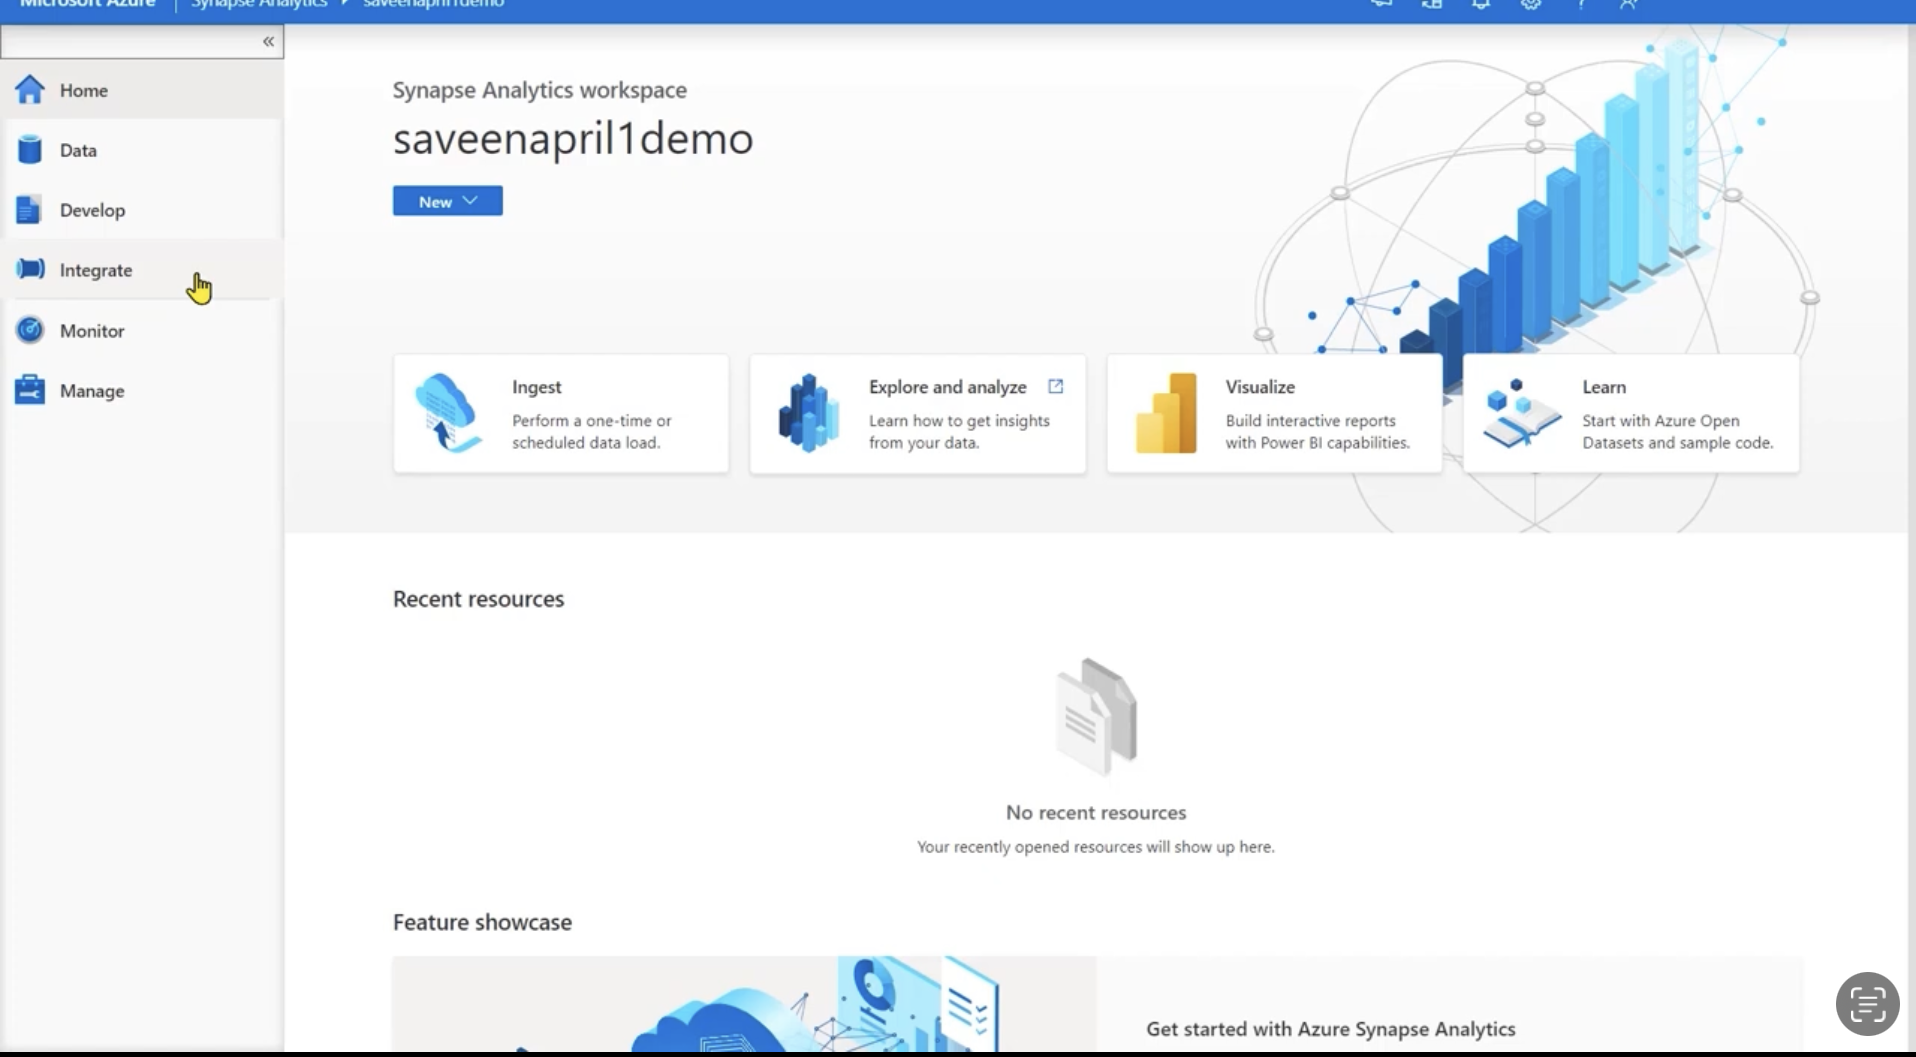
\includegraphics[scale = 0.2]{attachment/chapter_2/Scc108}
	\caption{Bsp.: Home Screen}
\end{figure}
Bei Home (Hub) kann eine individuelle Startseite angelegt werden.

\section{(Offen) Data (Hub)}
Über diesen Hub können alle verbunden (\textit{linked}) und Workspace Daten eingesehen werden.

\begin{figure}[H]
	\centering
	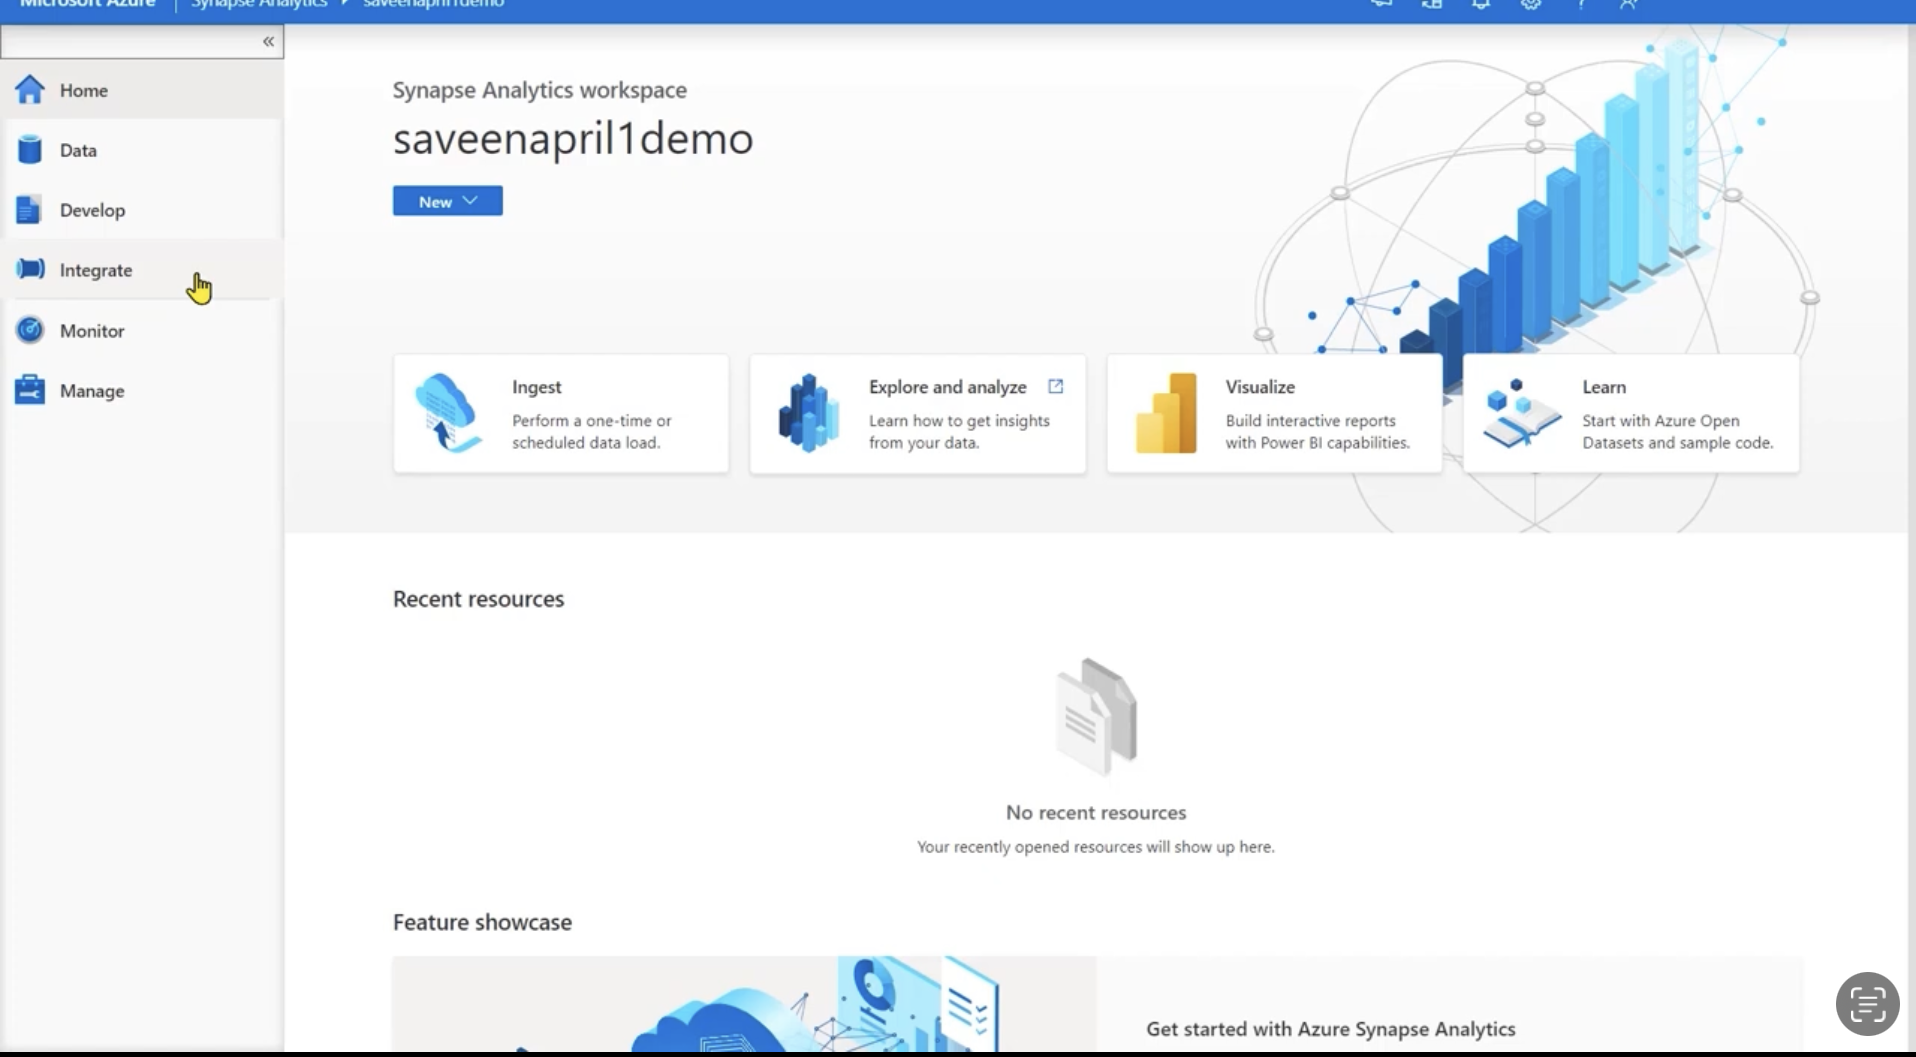
\includegraphics[scale = 0.2]{attachment/chapter_2/Scc108}
	\caption{Bsp.: Home Screen}
\end{figure}

Wenn ein System Daten erhält oder verarbeitet, welches in einem oder mehreren Dimensionen extrem vorliegen, spricht man von \textit{Big Data}.

\section{Lake Database}
\subsection{Concept}
Es handelt sich hier um ein weiteres Werkzeug, welches Struktur für Daten in einem \gls{ADL} bieten soll. Wie unter \nameref{subsec_Unterschied_Blob_Storage} beschrieben, ist ein Data Lake dafür gedacht, dass Daten ohne jegliche Struktur dort gesammelt werden soll. Das Werkzeug \textit{Lake Database} soll die Relationsstruktur einer Datenbank wie in \textit{SQL} bieten und gleichzeitig Zugriff auf den Lake besitzen.
\begin{figure}[H]
	\centering
	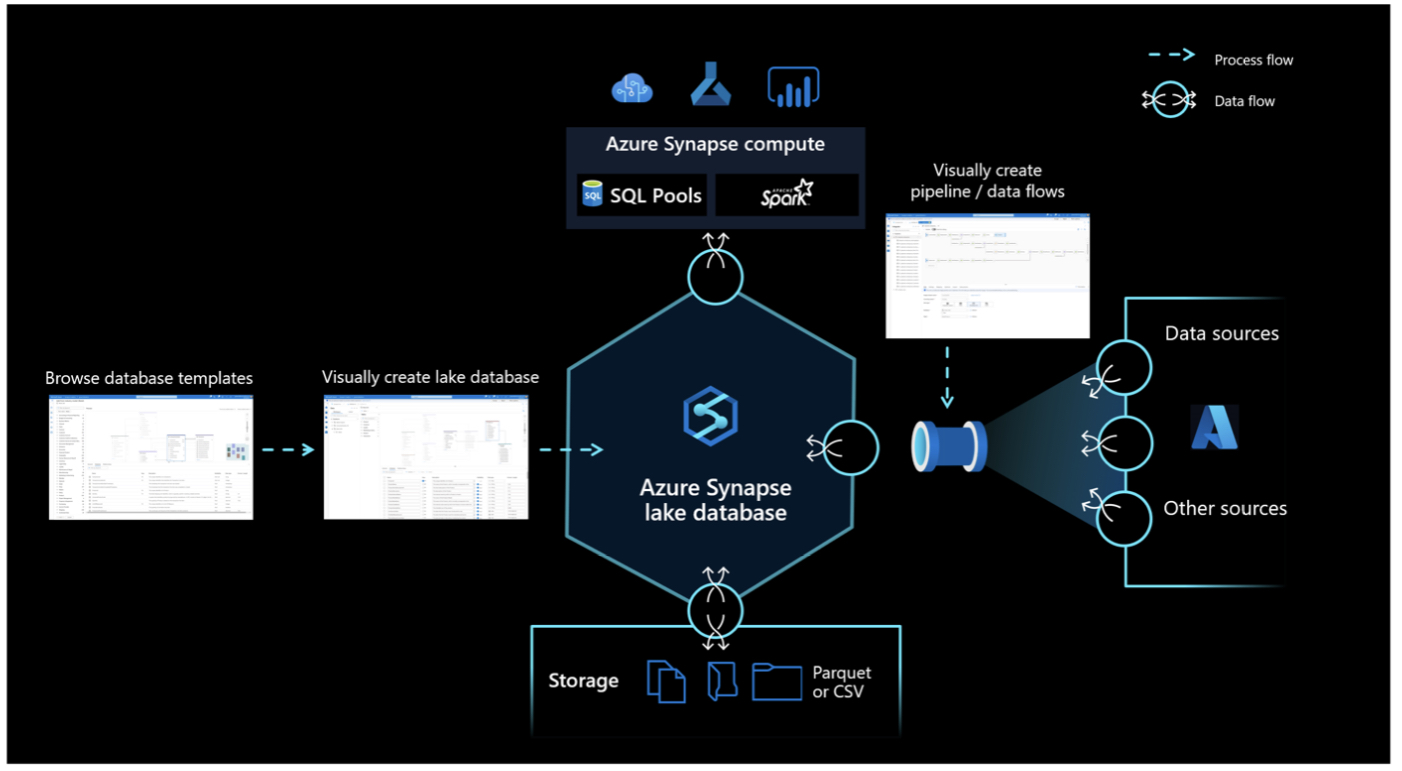
\includegraphics[scale = 0.2]{attachment/chapter_2/Scc137}
	\caption{Verbindungsstück Lake Database}
\end{figure}

Wie in der Übersicht zu sehen ist, die \textit{Lake Database} mit den anderen Zugängen von Synapse verbunden.


\subsection{Exersice: Combine Data with Mapping Tool}
Das \textit{Mapping Tool (Preview)} hilft den \gls{ETL} Prozess für einen Dataflow mit einer entsprechenden Pipeline zu vereinfachen.\\ 

Es um die Erstellung eines Datamodell, welche mit Daten $"$befüllt$"$ wird und dann als Database für den Lake verwendet werden kann. Mit dem Werkzeug \textit{Lake Database} soll die Komplexität eines Lake reduziert werden und Daten des Lake leichter zugänglich gemacht werden könne.

\href{https://learn.microsoft.com/en-us/azure/synapse-analytics/database-designer/concepts-lake-database}{Quelle}

\paragraph{Create Data Modell}
Für die Erstellung von Datensätzen steht die \textit{Curated database} zur Verfügung. Die andere erstellten sind entweder \textit{default} oder wurde über Spark SQL Skript erstellt.
\begin{figure}[H]
	\centering
	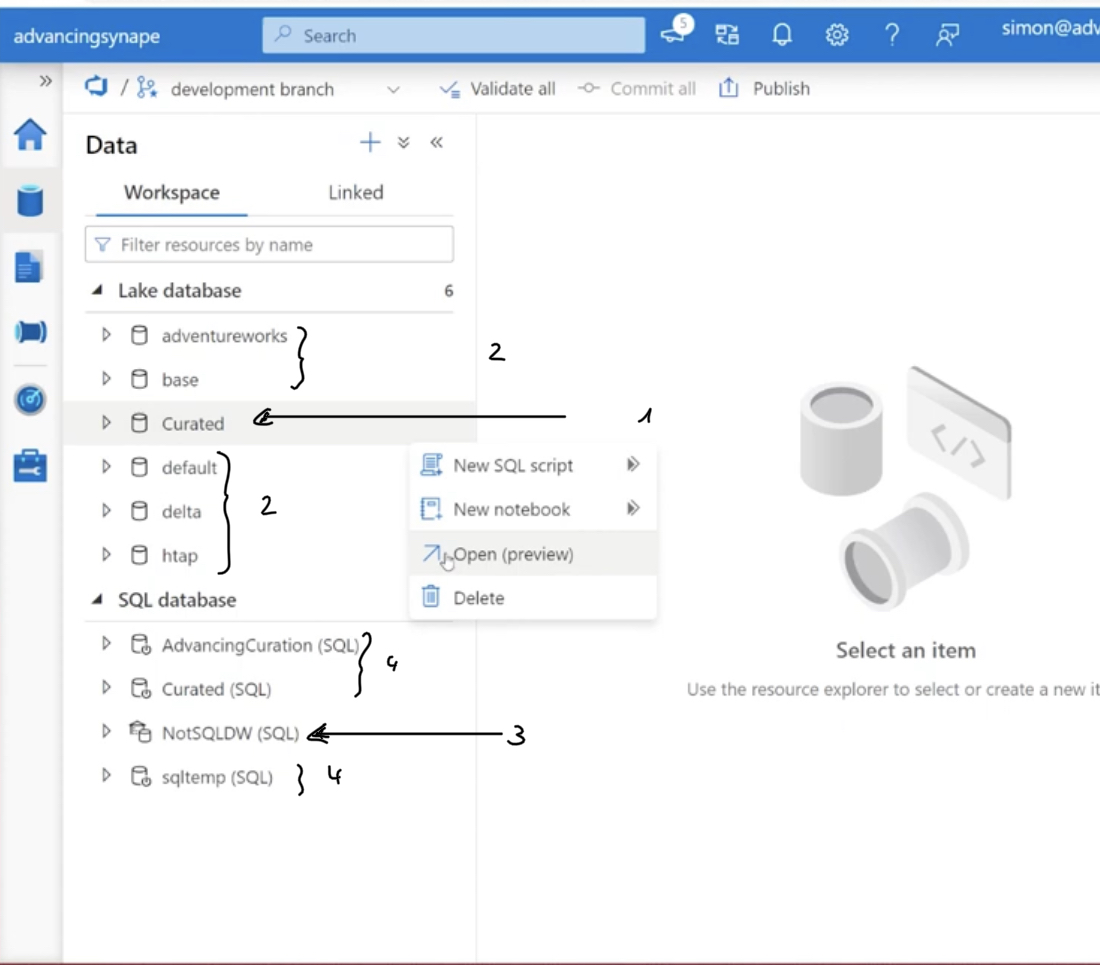
\includegraphics[scale = 0.2]{attachment/chapter_2/Scc138}
		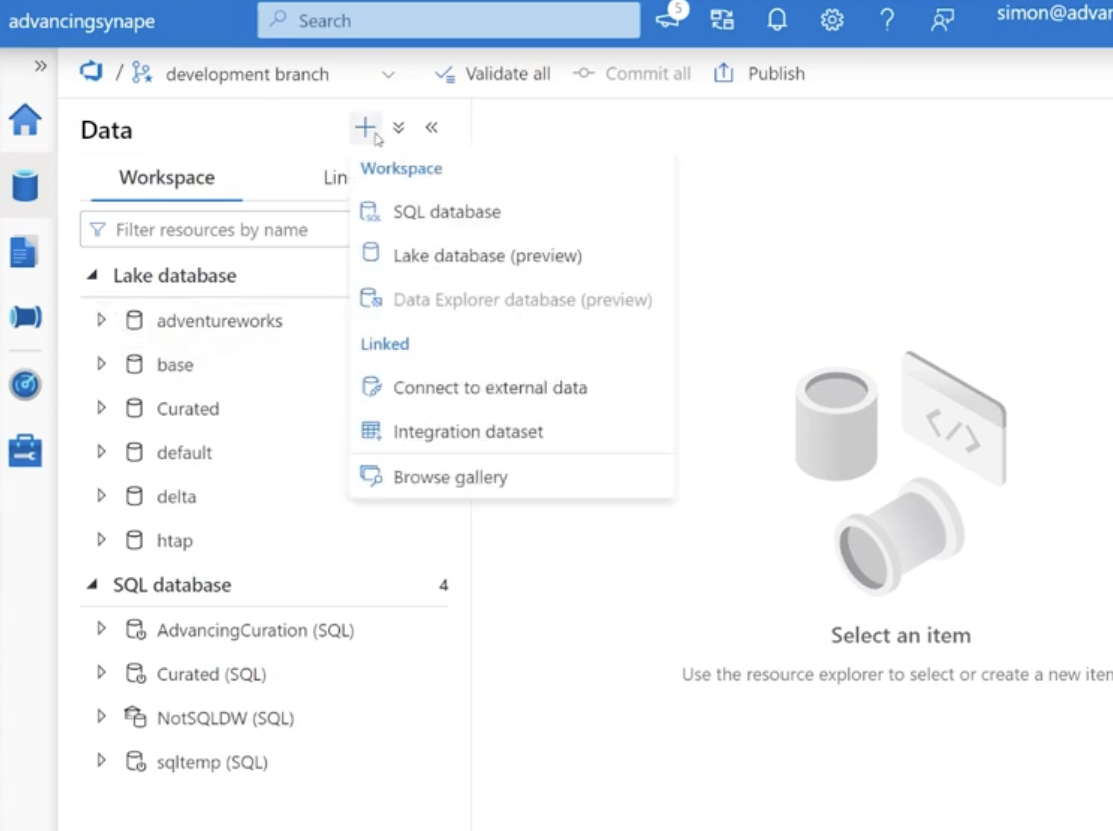
\includegraphics[scale = 0.2]{attachment/chapter_2/Scc139}
	\caption{Workspace/ Lake database/Create Lake database}
\end{figure}

\begin{itemize}
	\item 1 - Synapse Lake database
	\item 2 - Spark Database created with \gls{SQL} Skript
	\item 3 - Serverless \gls{SQL} Pool
	\item 4 - Dedicated \gls{SQL} Pool
\end{itemize}

Der \textit{Lake database} wird über das Menü geöffnet. Hier in Preview). Über das Menü \textit{Open (Preview)} wird das die Oberfläche für die Datenbank Modellierung (Database Designer) geöffnet.

\begin{figure}[H]
	\centering
	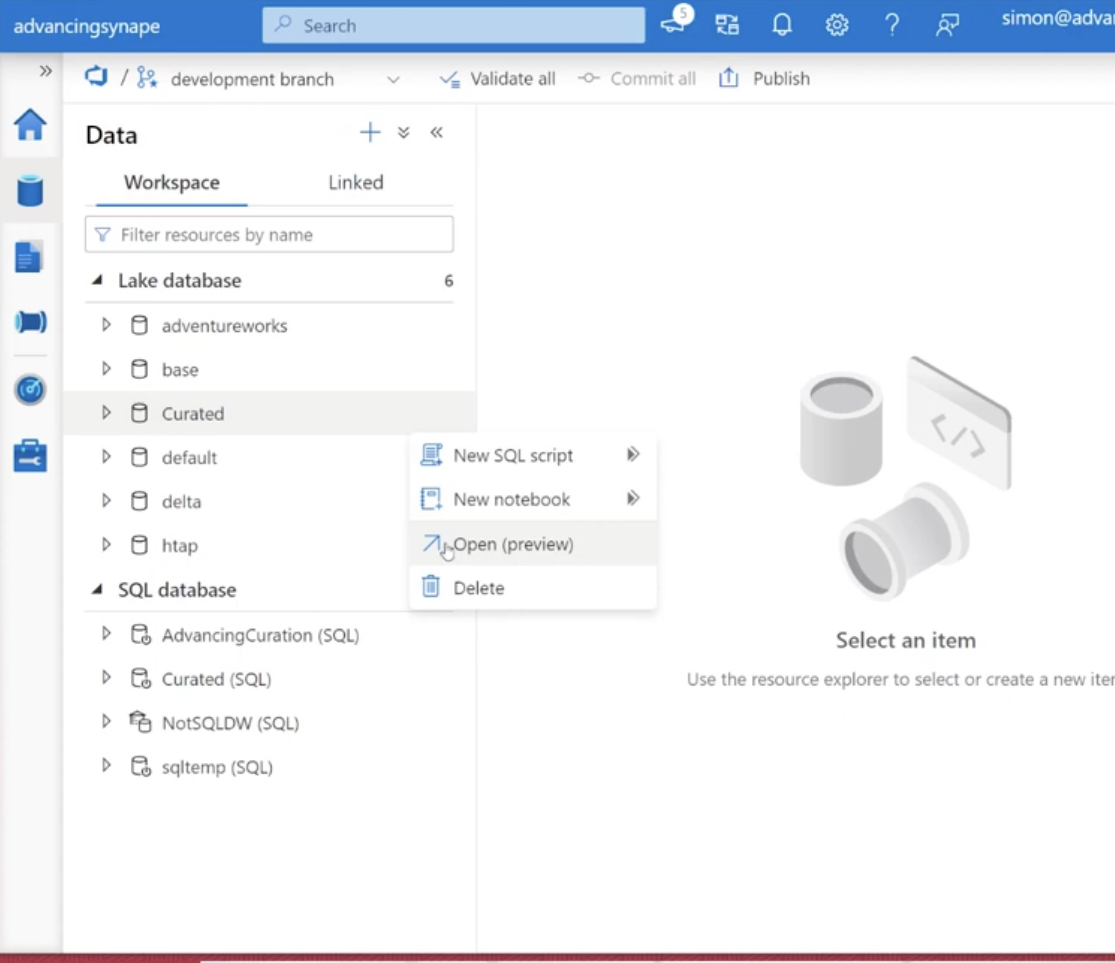
\includegraphics[scale = 0.2]{attachment/chapter_2/Scc140}
		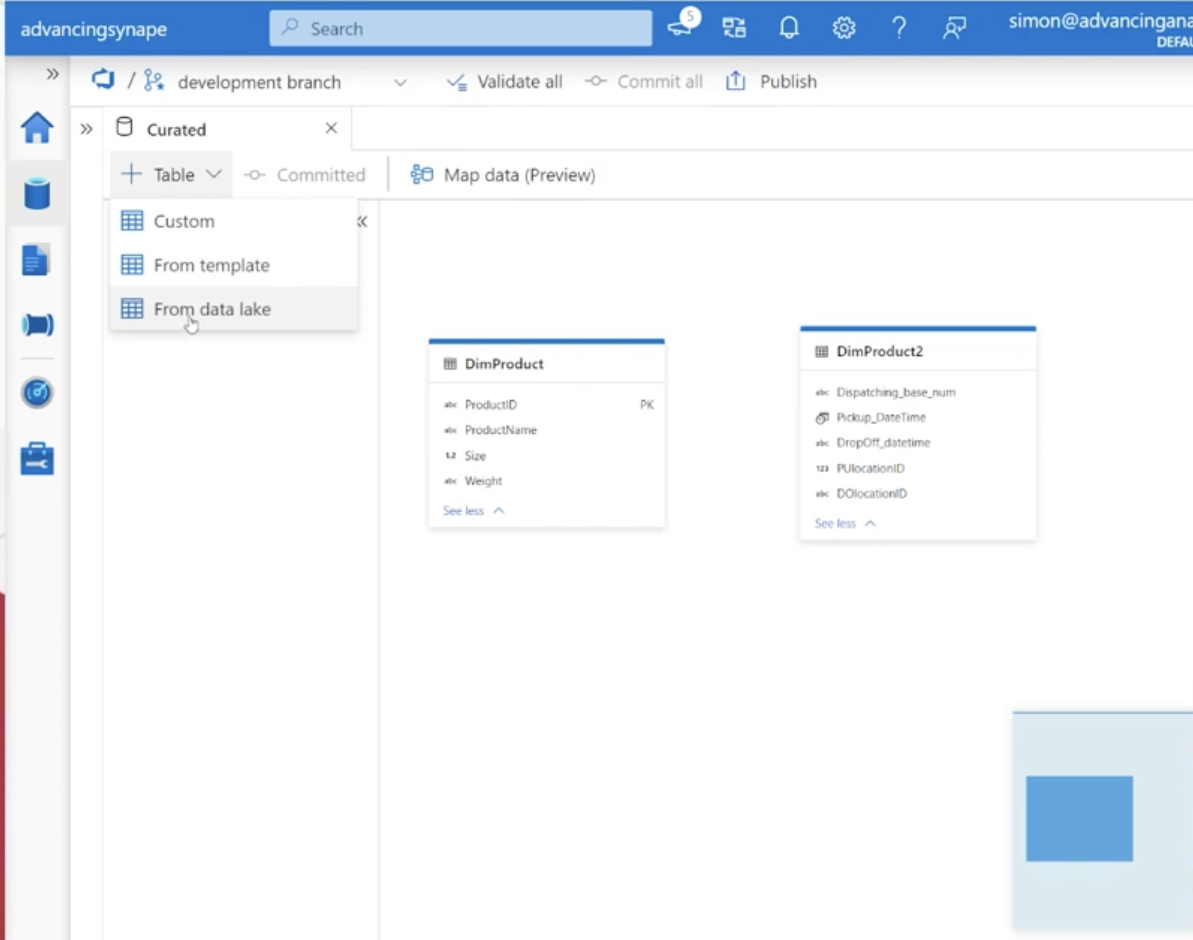
\includegraphics[scale = 0.2]{attachment/chapter_2/Scc142}
	\caption{Open data model tool} 
\end{figure}

Hier sieht mal gleich zwei Tabellen. Zum einen \textit{DimProduct} und \textit{DimProduct2}. Diese können entweder entweder manuell erstellt werden oder als Schema Kopien von einem Template oder einer Tabelle aus dem Data Lake erstellt werden.\\

Hier wird eine neue Tabelle erstellt. Die Spalten und nähere Konfigurationen für das Datenmodell werden hier festgelegt. Unter General wird der Speicher- pfad und das -format für die Tabelle festgelegt. Es wird nämlich hier nicht nur eine Datenmodell erstellt, sondern auch die Bereitstellung dieses ermöglicht. Dies bedeutet, das Datenmodell ist zwar logisch angelegt, die Daten des Modelles werden aber wieder direkt in den Lake gespeichert.

\begin{figure}[H]
	\centering
	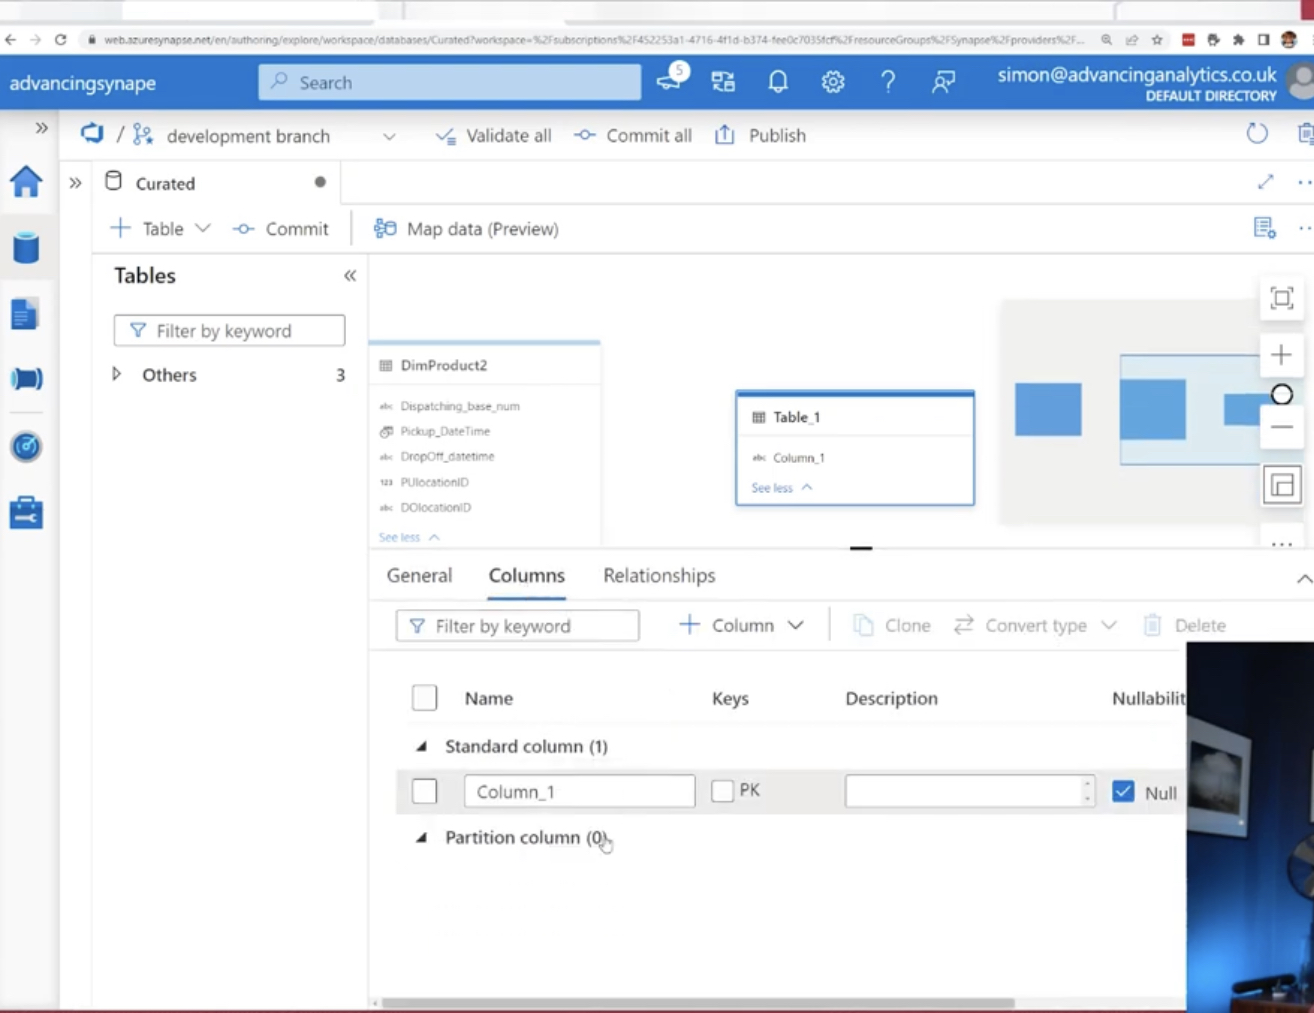
\includegraphics[scale = 0.2]{attachment/chapter_2/Scc141}
		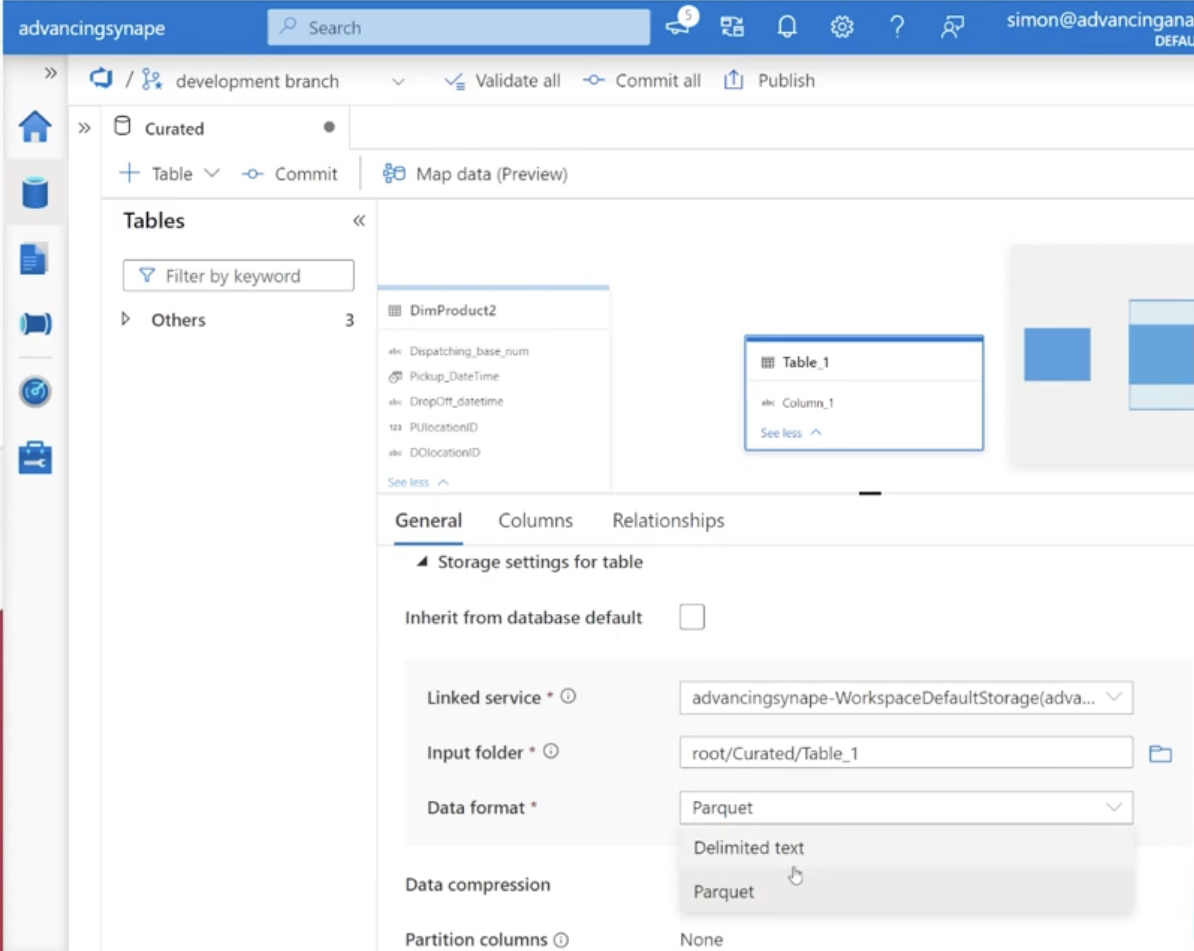
\includegraphics[scale = 0.2]{attachment/chapter_2/Scc143}
	\caption{Create Own Table}
\end{figure}

\paragraph{Create Mapping - Populated Data}
Is the data model created, then the source, where the data is stored is set. The next stepp is to find data to get into the data model.

\begin{figure}[H]
	\centering
	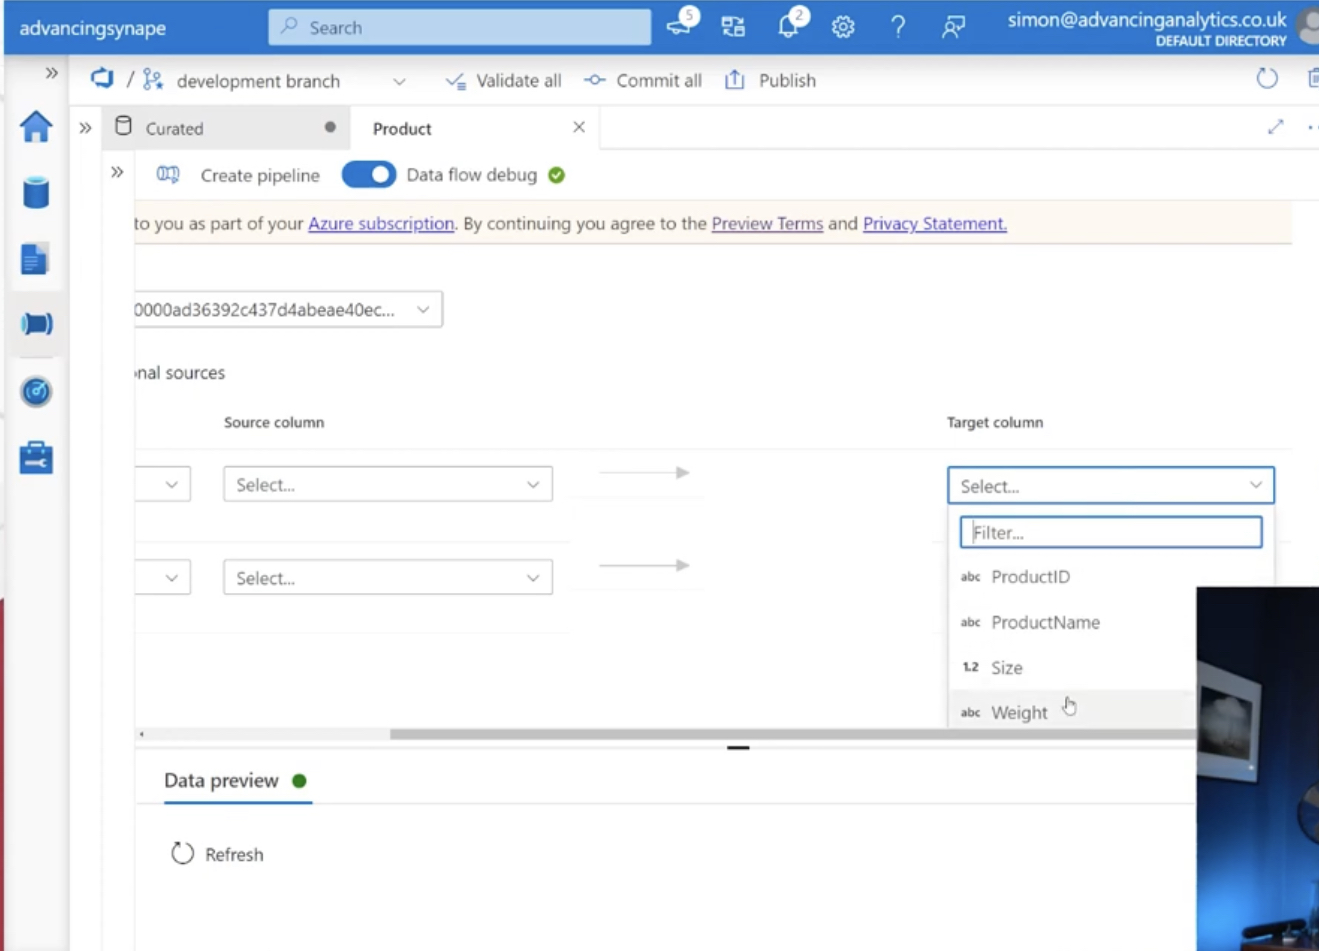
\includegraphics[scale = 0.2]{attachment/chapter_2/Scc145}
	\caption{Map data GUI}
\end{figure}

Wenn die Quelle für die Daten angelegt ist, wird eine 
\begin{itemize}
	\item Parent-Pipeline erstellt, welche eine Verschneidung mehrerer Datenquellen zulassen würde, 
	\item eine Child-Pipeline, welche für die hier eine ausgewählte Datenquelle erstellt wurde und
	\item ein Dataflow für die eine Datenquelle.
\end{itemize}

\begin{figure}[H]
	\centering
	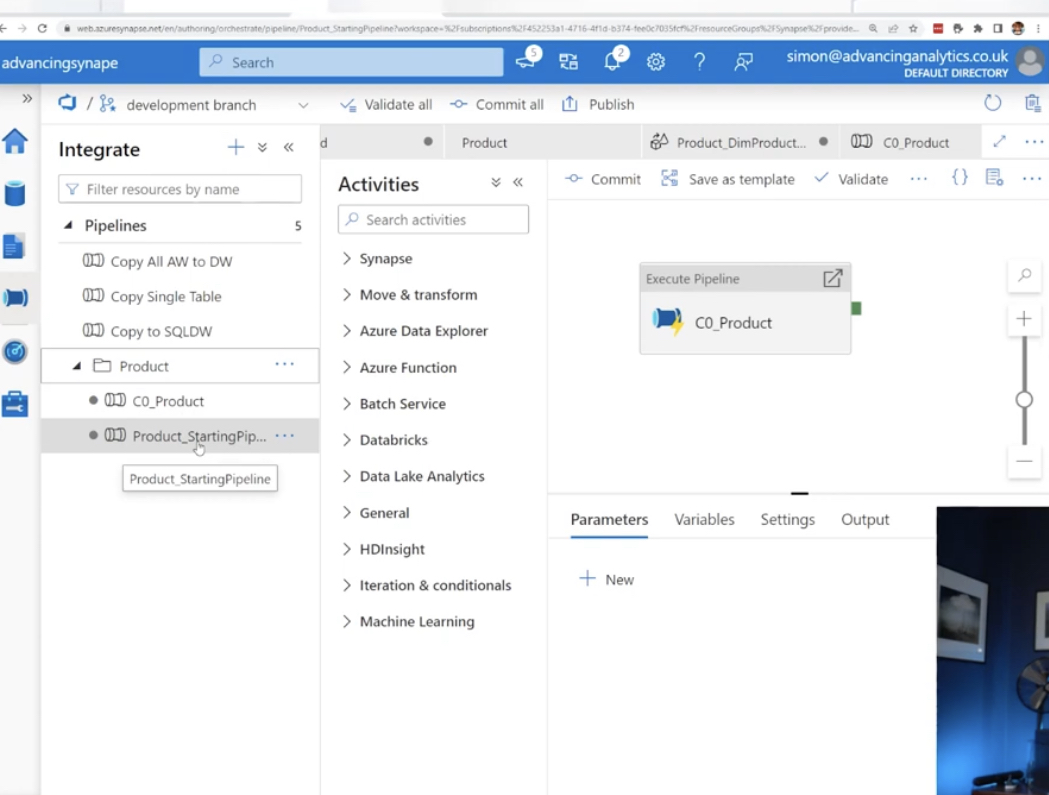
\includegraphics[scale = 0.2]{attachment/chapter_2/Scc146}
	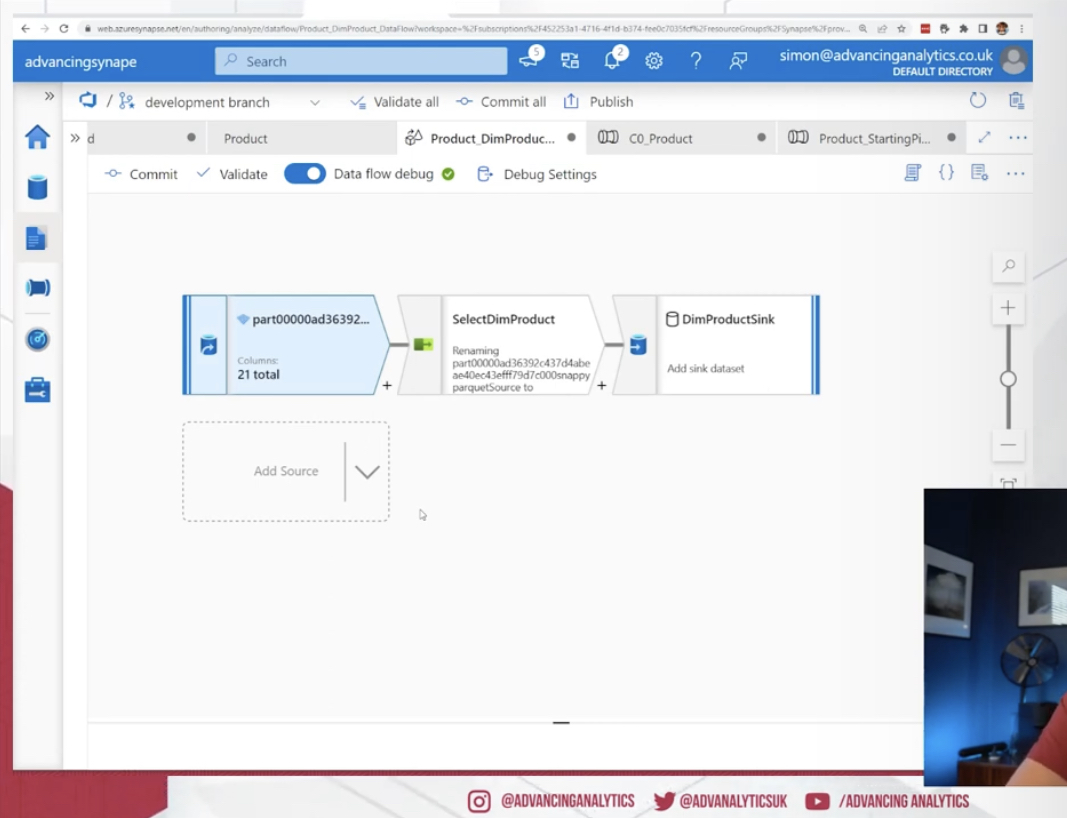
\includegraphics[scale = 0.2]{attachment/chapter_2/Scc147}
	\caption{Created Pipelines and Dataflow}
\end{figure}

Es werden unter dem Dataflow eine Data Import, Select und Store Aktivität angelegt. In diesem Beispiel werden die Daten aus dem Lake geholt und in das logische Modell geladen und dann wieder in den Lake geschoben.

\paragraph{Configure underlining Dataflow}
Entweder verweist das Datenmodell auf bestehenden Date oder enthält nur eine Leere Hülle (Schema) mit einen Speicherpfad. In beiden Fälle ist das Ziel mit Mapping, neue Daten in der richtigen Form und Format in das aufgezeigt Datenmodell kontinuierlich oder einmalig zu befühlen.\\

Als erstes wird die Quelle definiert, von wo die Daten her übernommen werden. Mit dem Mapping Tool können nur spezifische Dateien ausgewählt werden. Dies kann später im generierten Dataflow zu einen Pfad Verzeichnis geändert werden.
\begin{figure}[H]
	\centering
	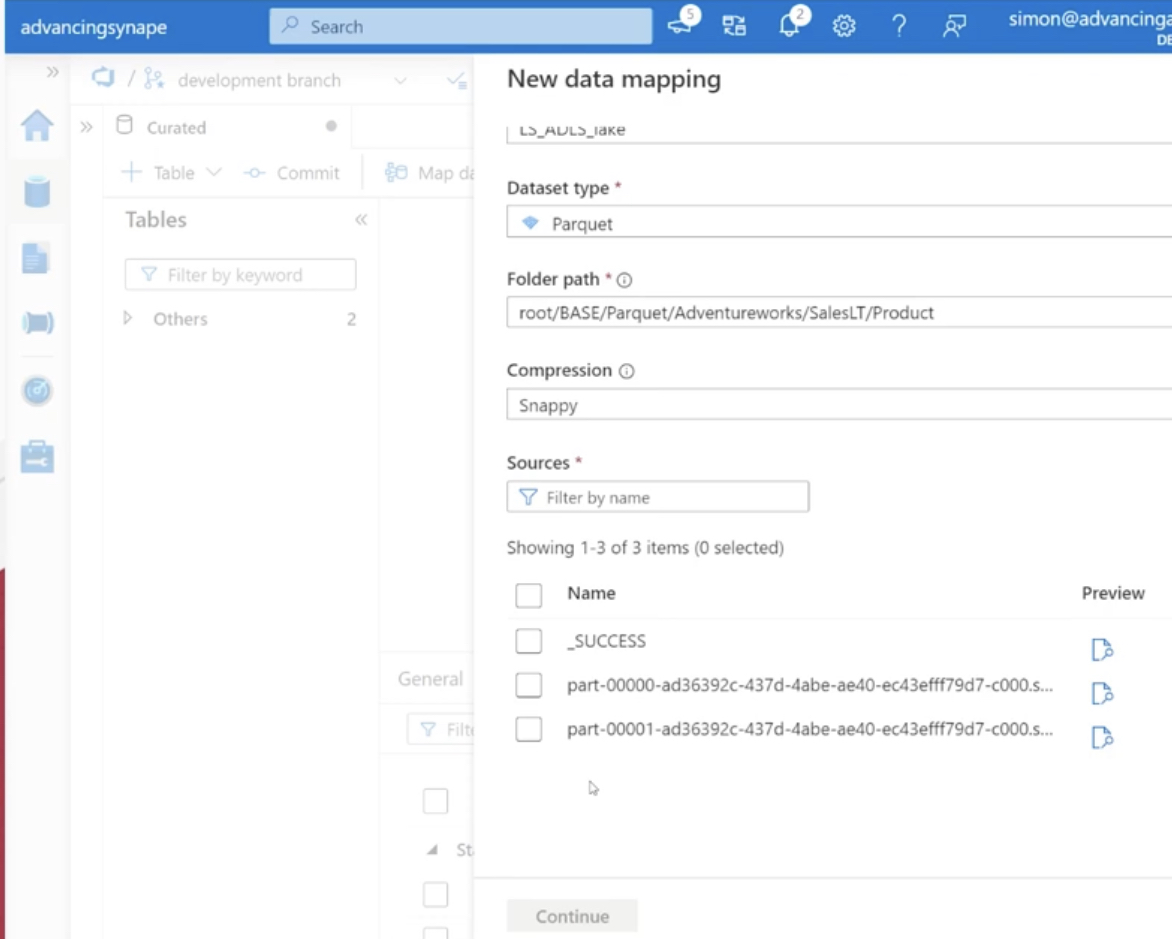
\includegraphics[scale = 0.2]{attachment/chapter_2/Scc144}
	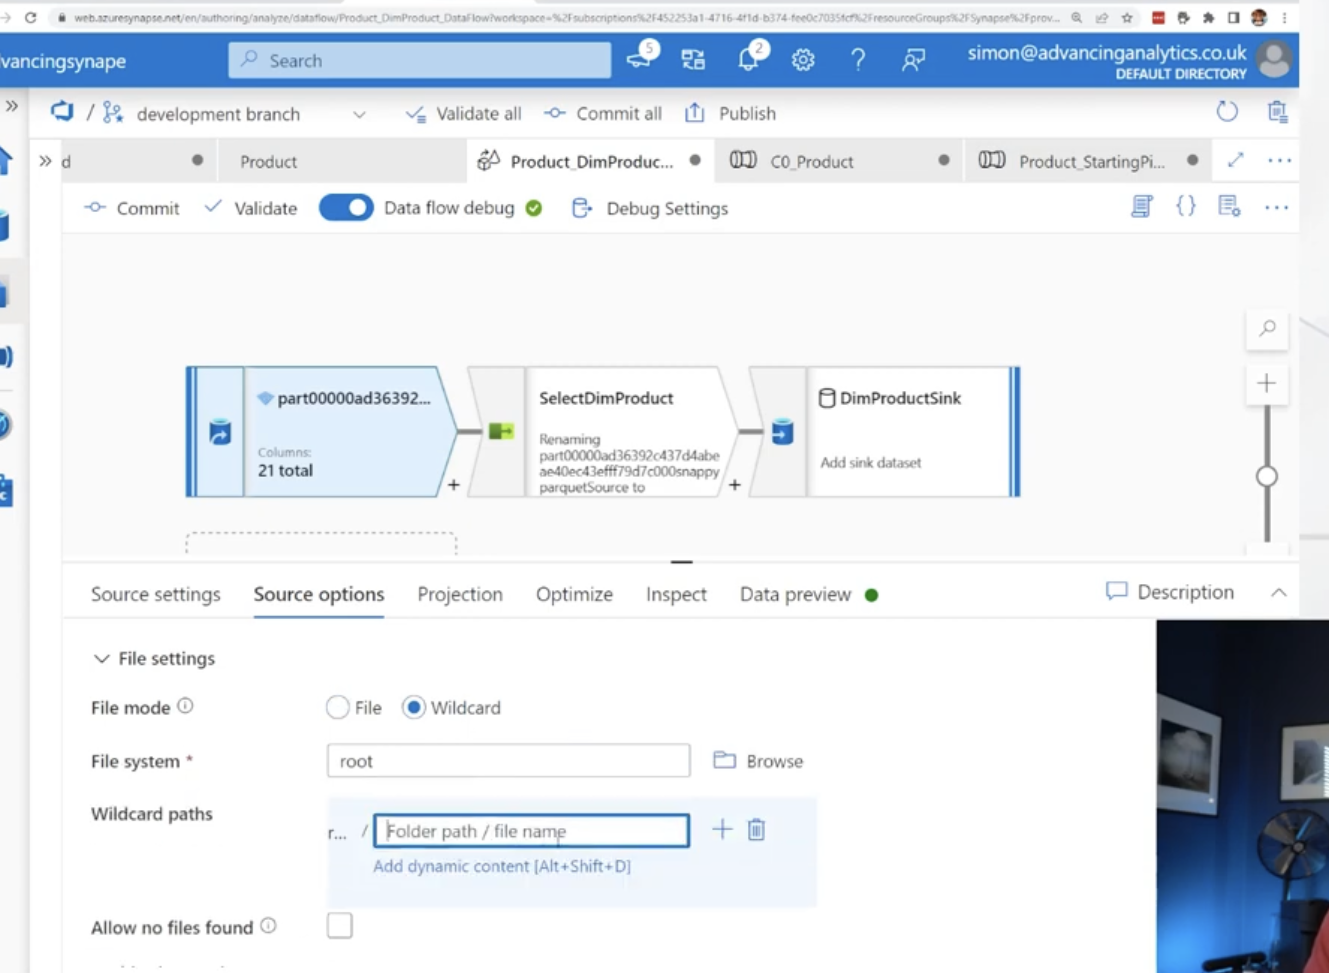
\includegraphics[scale = 0.2]{attachment/chapter_2/Scc149}
	\caption{Starting the Mapping Tool/ Modify later data flow}
\end{figure}


\section{CI/CD Workspaces}

\subsection{Übersicht}
Gegeben drei Synapse Workspaces
\begin{itemize}
	\item Develpment
	\item Test (UTA)
	\item Production
\end{itemize}
ist das Ziel mit dem Abschnitt zu beschreiben, wie eine Entwicklung von Code in der Entwicklungsumgebung aussehen kann, und diese dann zwischen Test und Produktion als Artifakt transportiert wird.\\

\subsection{Versionskontrolle}
Die Versionskontrolle erfolgt außschließlich über den \textit{Synapse Development Workspace}. Die Workspaces \textit{Test} und \textit{Production} werden nicht mit einem jeweiligen git Repository verbunden.\\

Im \textit{Test} und \textit{Produktions} Workspace wird nur über \textit{Synpase live} gearbeitet.

\subsection{Create a Artifact}
\paragraph{Publishing}
Über die Versionskontrolle über \textit{Azure DevOps Repo} wird der \textit{master} Branch mit den neusten Änderungen befüllt. Über Synapse selbst wird ein \textit{Artifact} erstellt, welches über \textit{Publishing} ausgewiesen wird.

\begin{figure}[H]
	\centering
	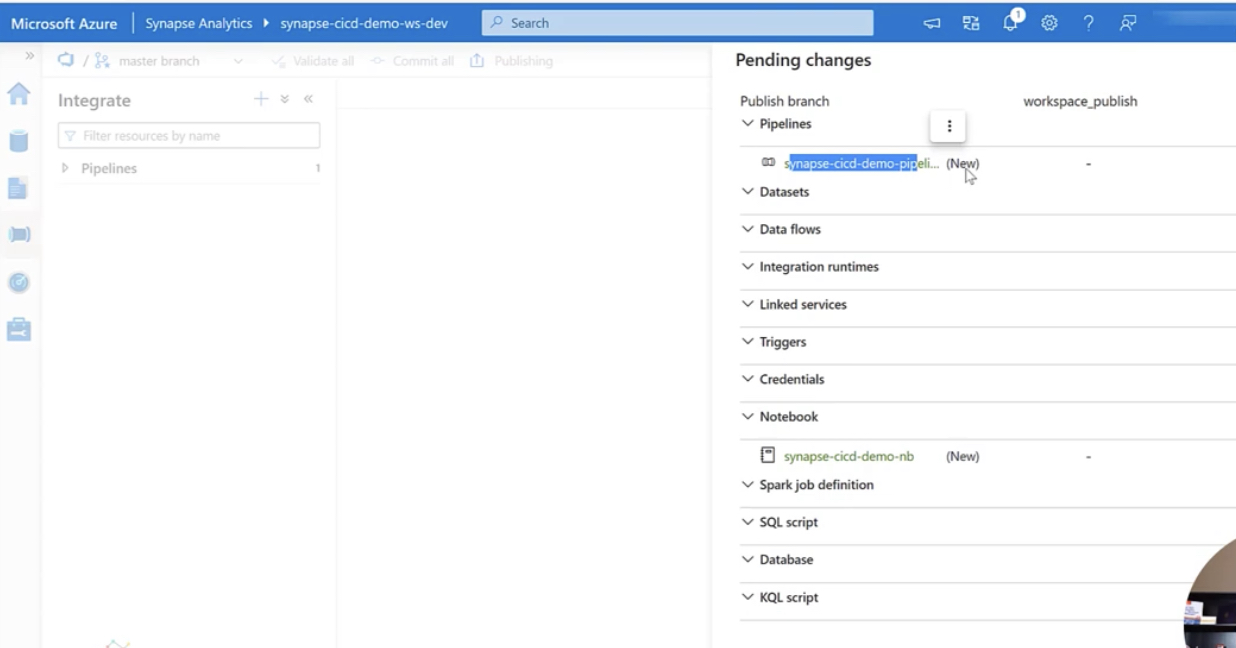
\includegraphics[scale = 0.2]{attachment/chapter_2/Scc151}
	\caption{Publishing Artifact to workspace branch} 
\end{figure}

Diese Anzeige erscheint, wenn der \textit{Publishing} Button direkt in Synapse gedrückt wird. Es wird angezeigt, welche Änderungen vorgenommen wurden. Wir oben angezeigt, wird von dem \textit{master} branch in den \textit{workspace publish} branch committet. \\

\textbf{Achtung:} Es werden nicht der Code aus master in den workspace publish branch gemergt. Es wird in dem Prozess ein Artifakt erstellt, welches abgelegt wird.


\paragraph{workspace Branch}
Im Workspace Branch wird ein 
\begin{itemize}
	\item Template
	\item und eine Parameter Konfiguration
\end{itemize}

hinterlegt.

\begin{figure}[H]
	\centering
	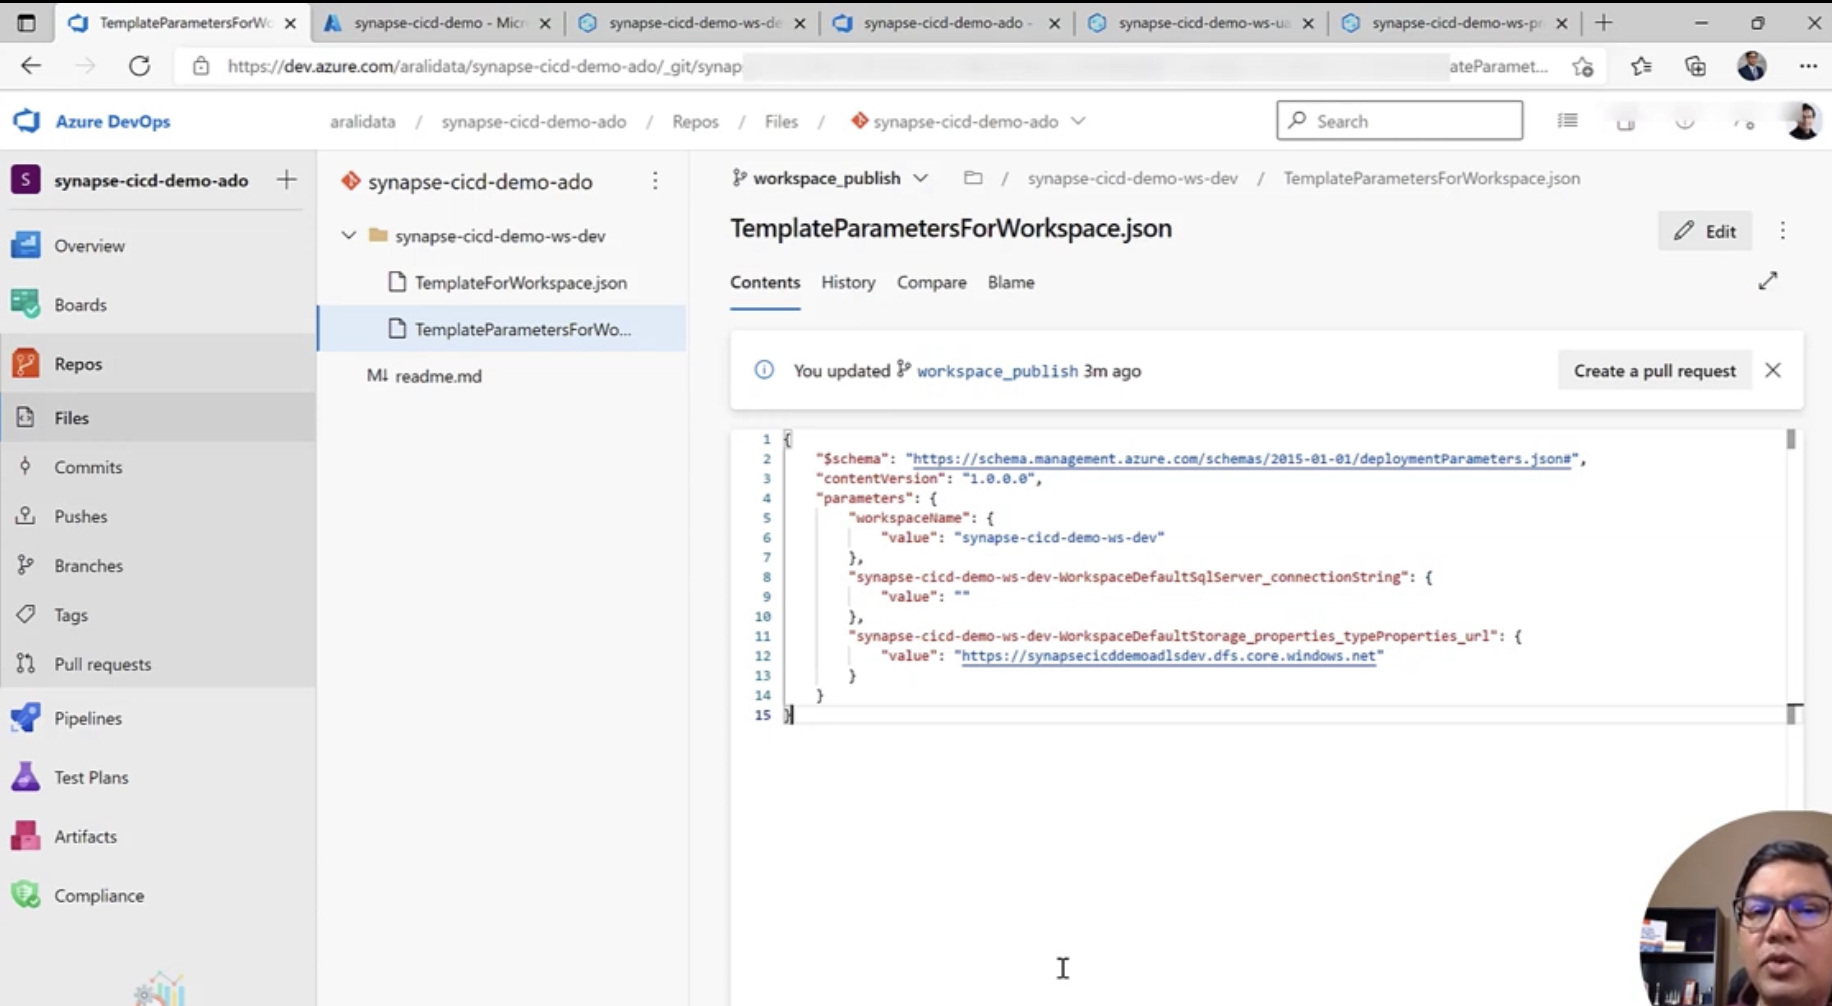
\includegraphics[scale = 0.2]{attachment/chapter_2/Scc152}
	\caption{Repository Artifacte Branch} 
\end{figure}

\subsection{Release Pipeline}
\subsubsection{Create}\label{pap_Create_a_Release_Pipeline}
\paragraph{Set Up}
Über Azure DevOps Pipeline/Release wird eine Transport Werkzeug erzeugt, welches die Änderungen aus der \textit{Developer} Umgebung in die \textit{Test} Umgebung $"$deployed$"$.\\

Zum Anfang wird ein Artifact ausgewählt. In Fall von Synapse ist dies der neuste Stand des \textit{workspace branches} aus zuwählten Artifacts

\begin{figure}[H]
	\centering
	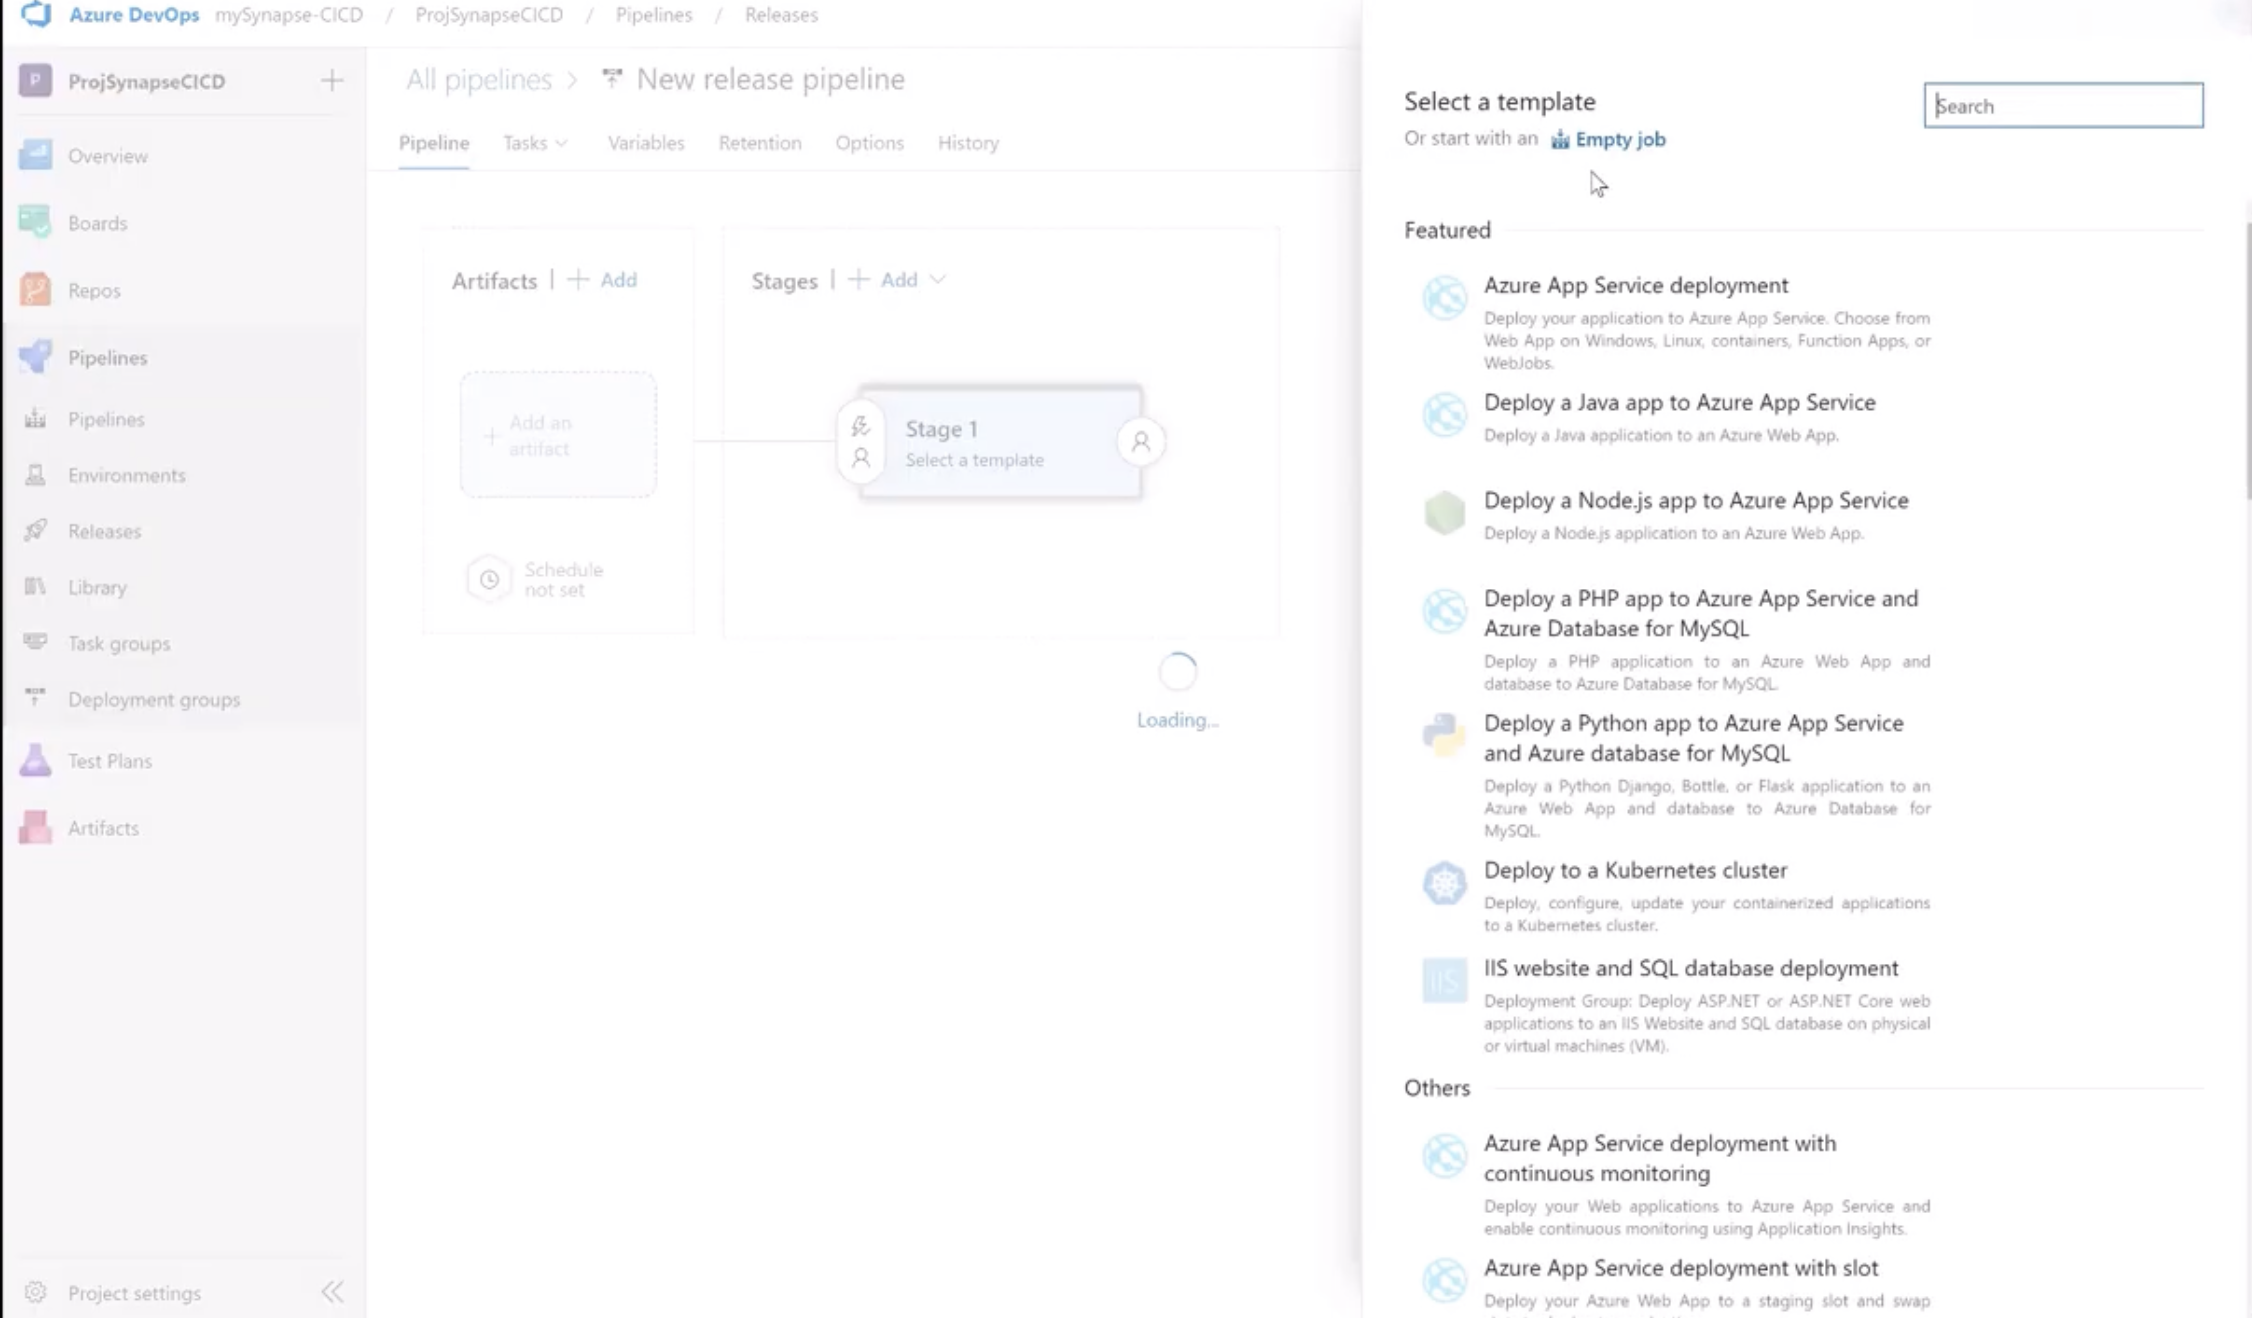
\includegraphics[scale = 0.2]{attachment/chapter_2/Scc153}
	\caption{Start Release Pipeline} 
\end{figure}

Die Konfiguration der \textit{Stage 1} erfolgt über ein eigenes Synapse Template.

\begin{figure}[H]
	\centering
	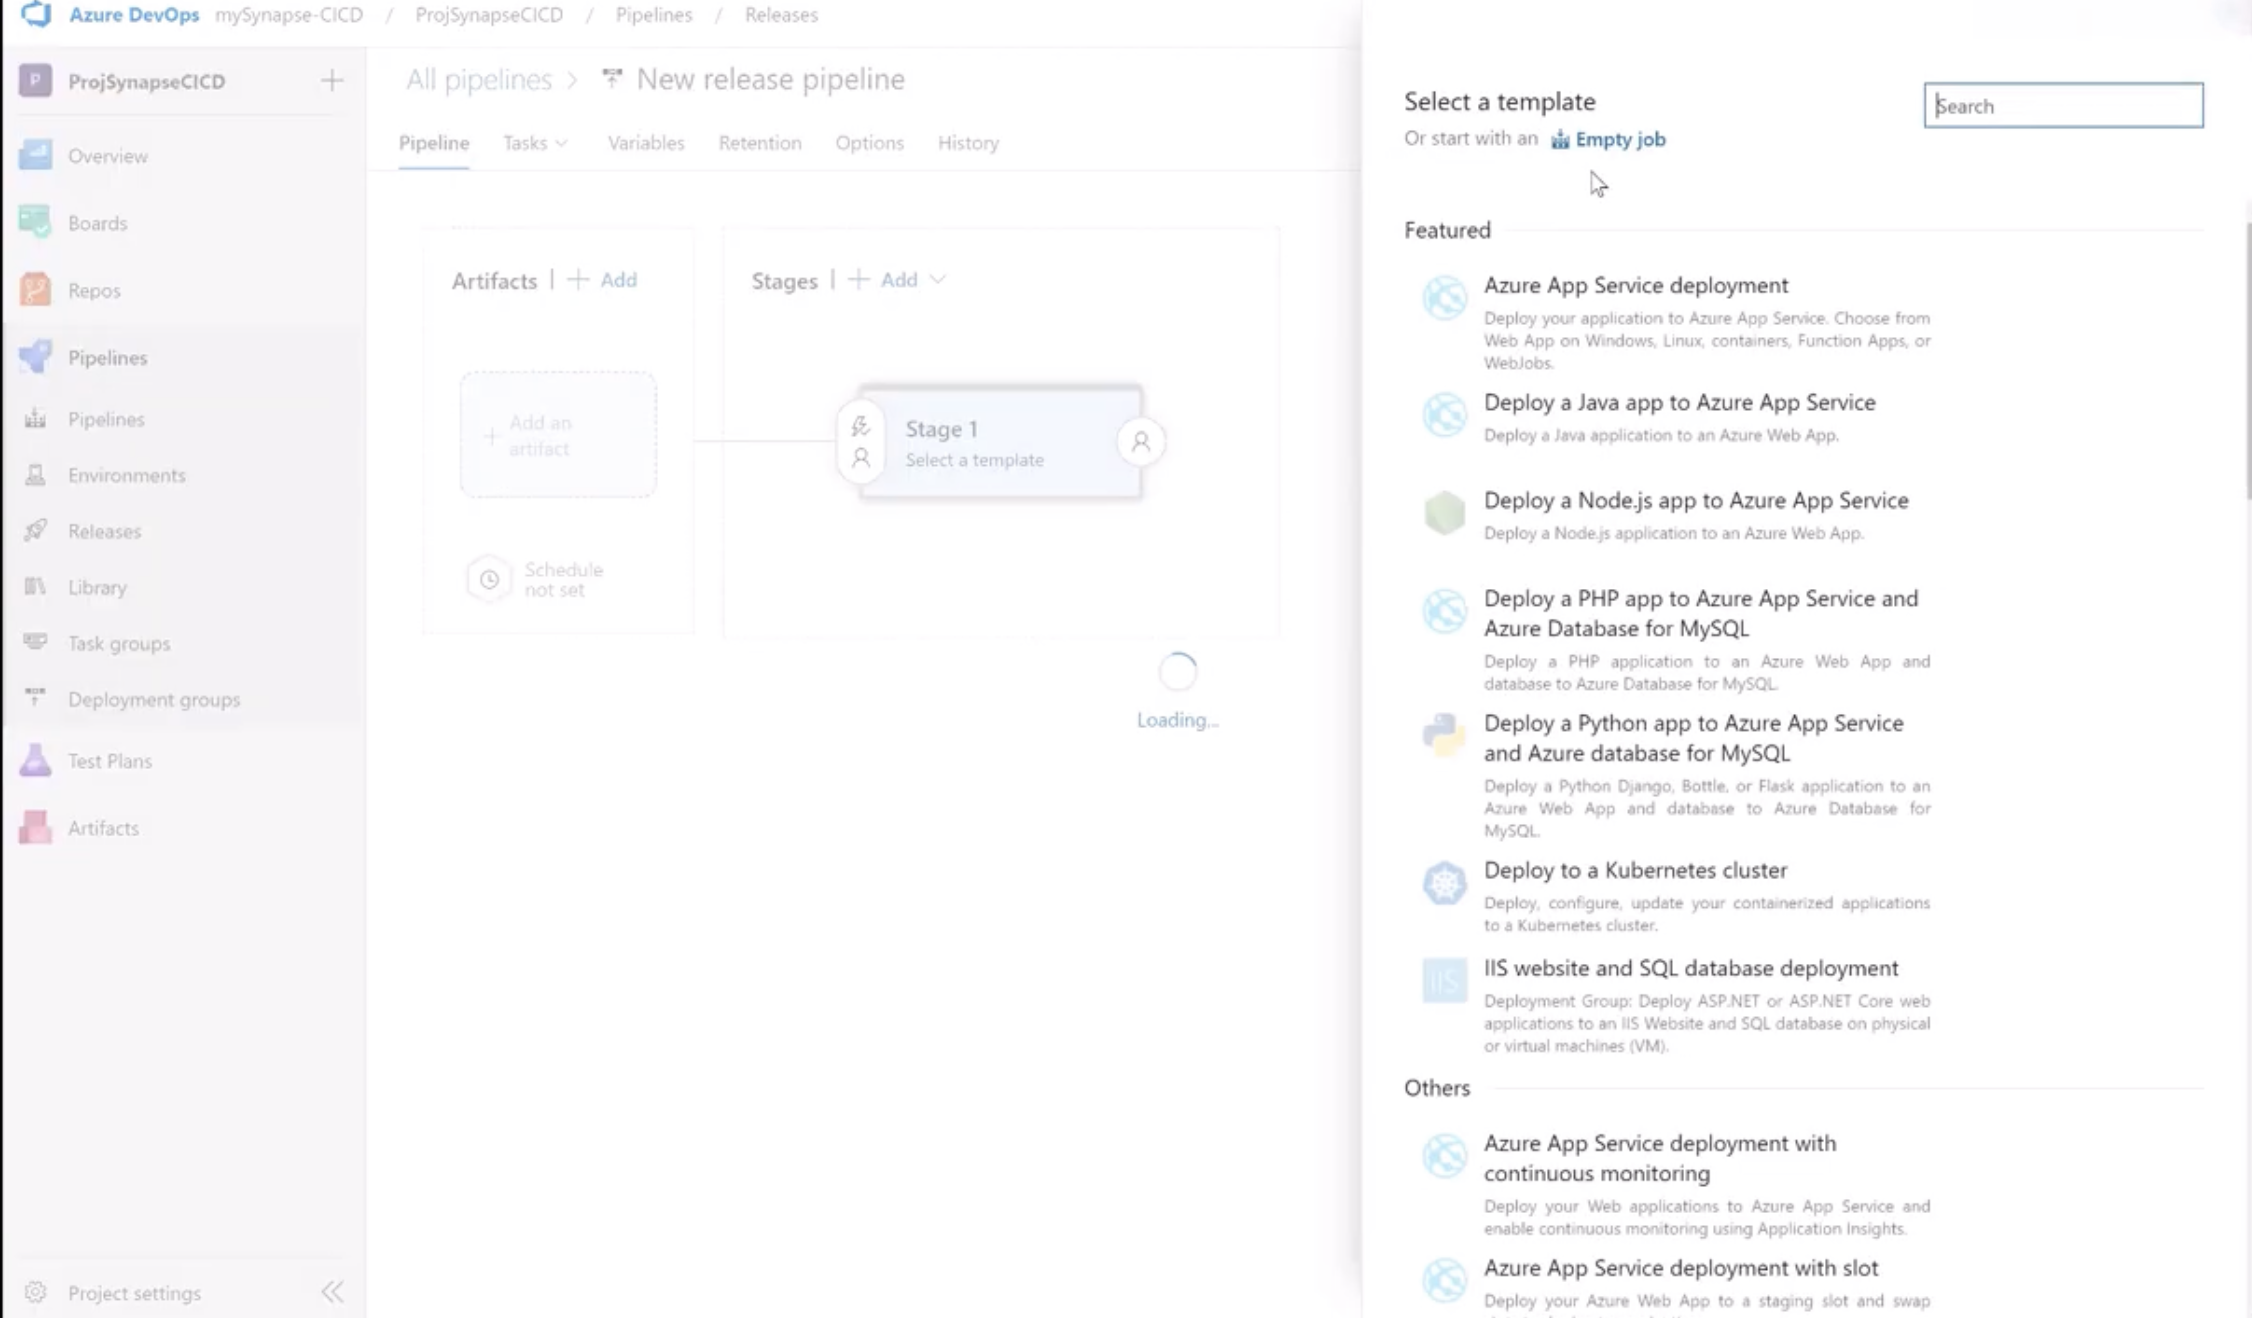
\includegraphics[scale = 0.2] {attachment/chapter_2/Scc153}
	\caption{Configuration Stage 1}
\end{figure}

\paragraph{Option: Archive Artifact}
Es gesteht auch die Möglichkeit, mehrere Schritte zu hinterlegen. 
Das Artifact kann auch archivert werden.

\subsubsection{Parmetrisieren}
\paragraph{Libary Variables}
Über die Bibliothek werden Variablen für die Pipeline hinterlegt.
\begin{figure}[H]
	\centering
	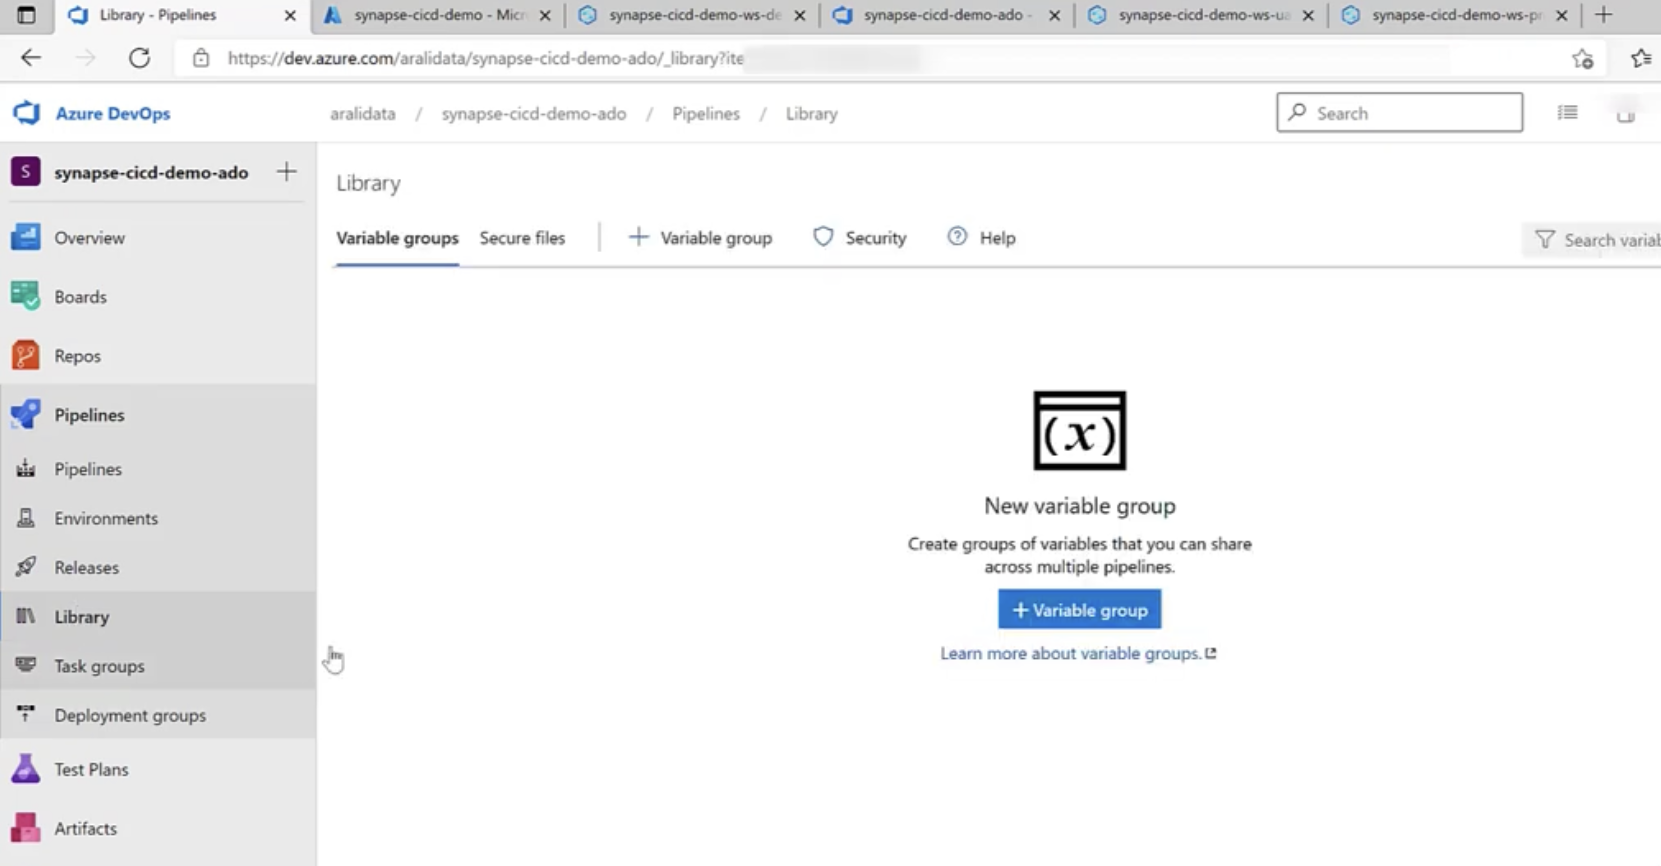
\includegraphics[scale = 0.2]{attachment/chapter_2/Scc155}
	\caption{Create Variable}
\end{figure}

In dem hier beschriebenen Fall, werden Variablen für verschiedene Umgebungen angelegt.

\begin{figure}[H]
	\centering
	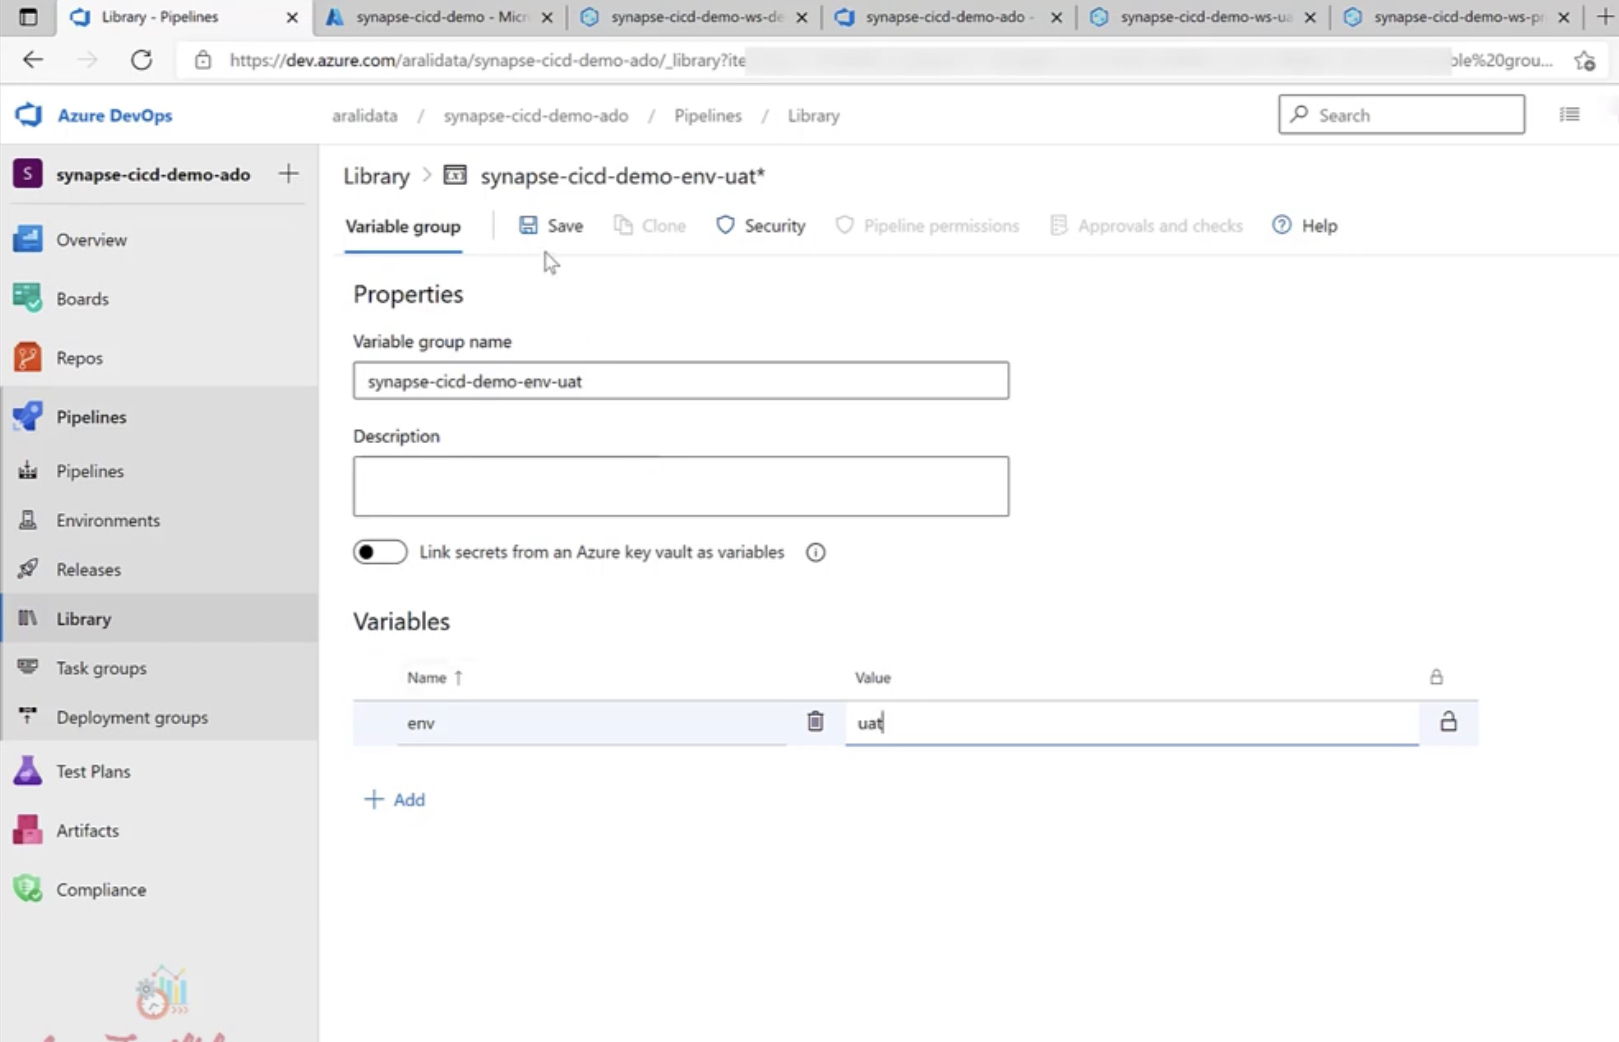
\includegraphics[scale = 0.2]{attachment/chapter_2/Scc156}
	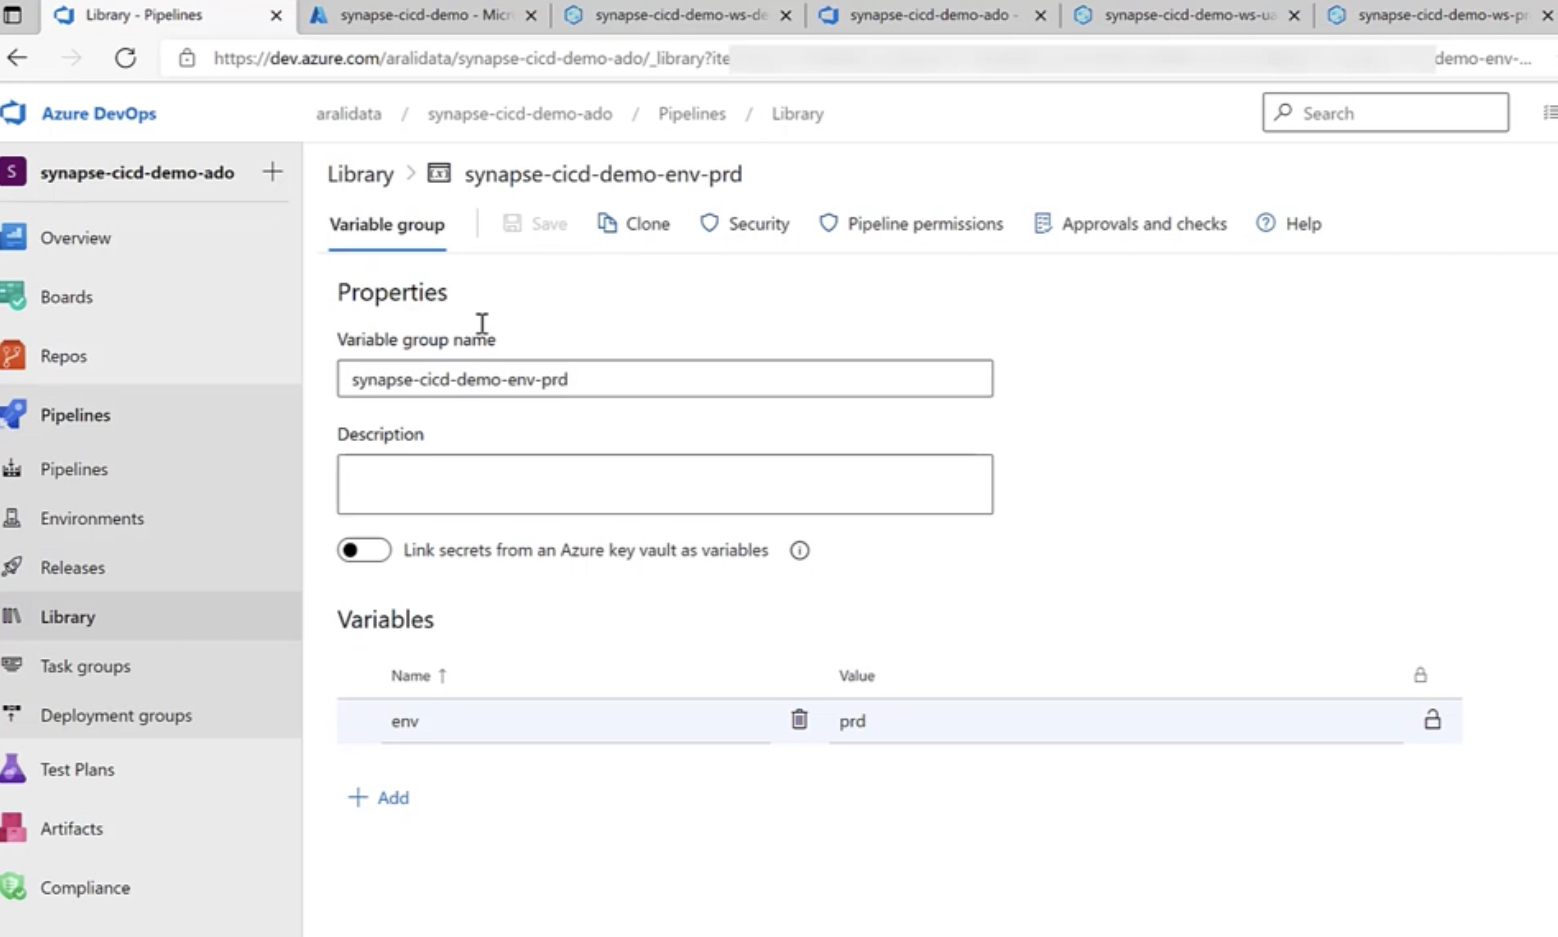
\includegraphics[scale = 0.2]{attachment/chapter_2/Scc157}
	\caption{Gruppierung von Variablen nach Umgebung}
\end{figure}

Für diese wurde die Variablen \textbf{env} mit dem Wert \textit{uta}/ \textit{prd} angelegt. Diese gibt die Namesabkürzung der Variablen wieder.

\paragraph{Pipeline Variable Mapping}
In der Pipeline wird ein Mapping benötigt. Dies verknüpft eine Pipeline Variable mit einer aus der Bibliothek oder kann auch einen eigenen manuellen Wert haben.

\begin{figure}[H]
	\centering
	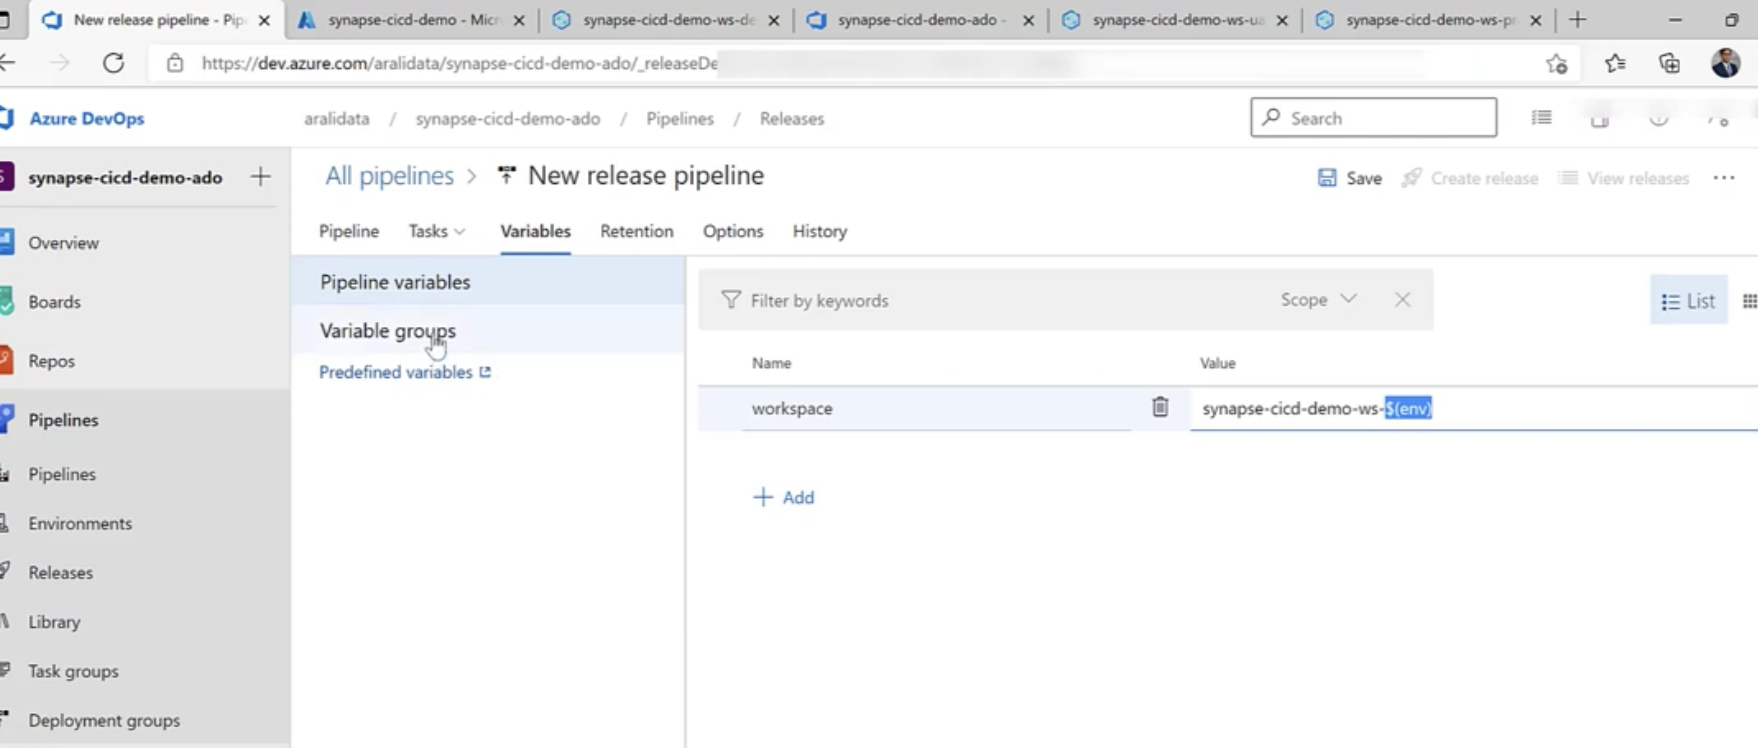
\includegraphics[scale = 0.2]{attachment/chapter_2/Scc158}
	\caption{Mapping of Variables}
\end{figure}

Die neu angelegt Variable, \textbf{workspace}, wird mit dem Variablen Gruppe \textit{synapse-cid-demo-ws-uta} und der Variablen \textit{env} verknüpft.\\

Wie bei Synapse selbst, wird eine Verlinkung benötigt. Diese kann für die gesamte Release Pipeline oder nur für den Stage gegeben werden.

\begin{figure}[H]
	\centering
	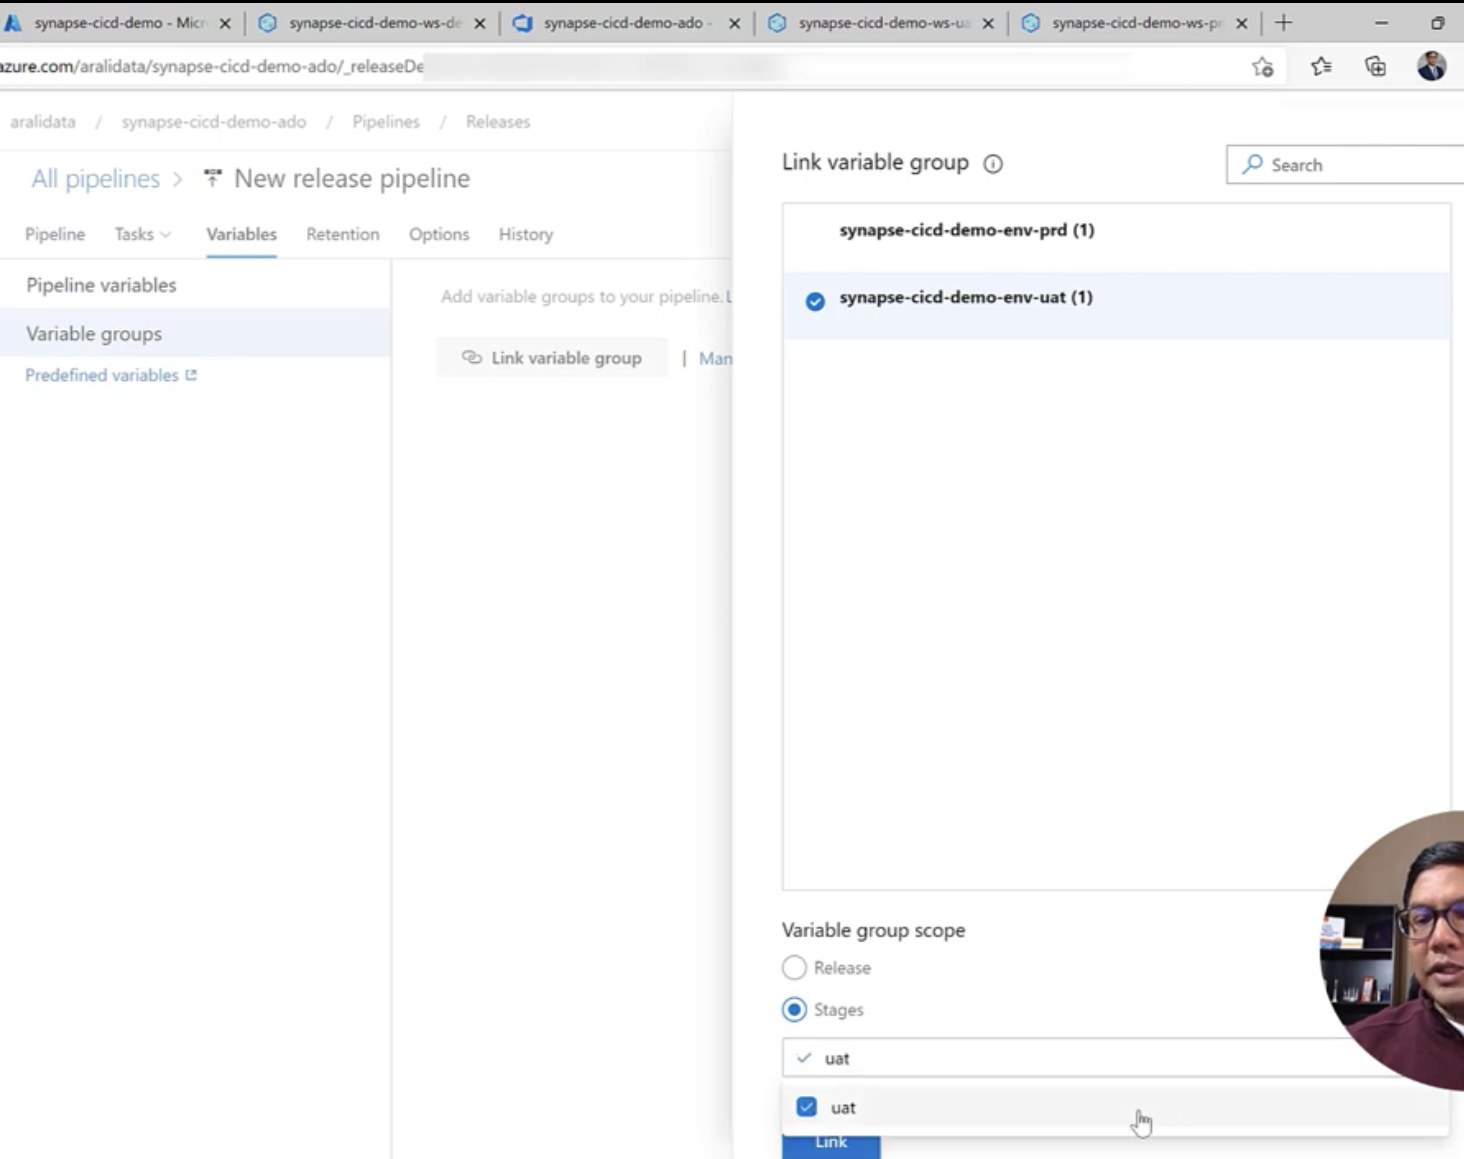
\includegraphics[scale = 0.2]{attachment/chapter_2/Scc160}
	\caption{Link Variable Group}
\end{figure}

\paragraph{Configuration of the task}
Wie unter \nameref{pap_Create_a_Release_Pipeline} zu sehen ist, wird aus dem Template die Konfiguration angelegt.

\begin{figure}[H]
	\centering
	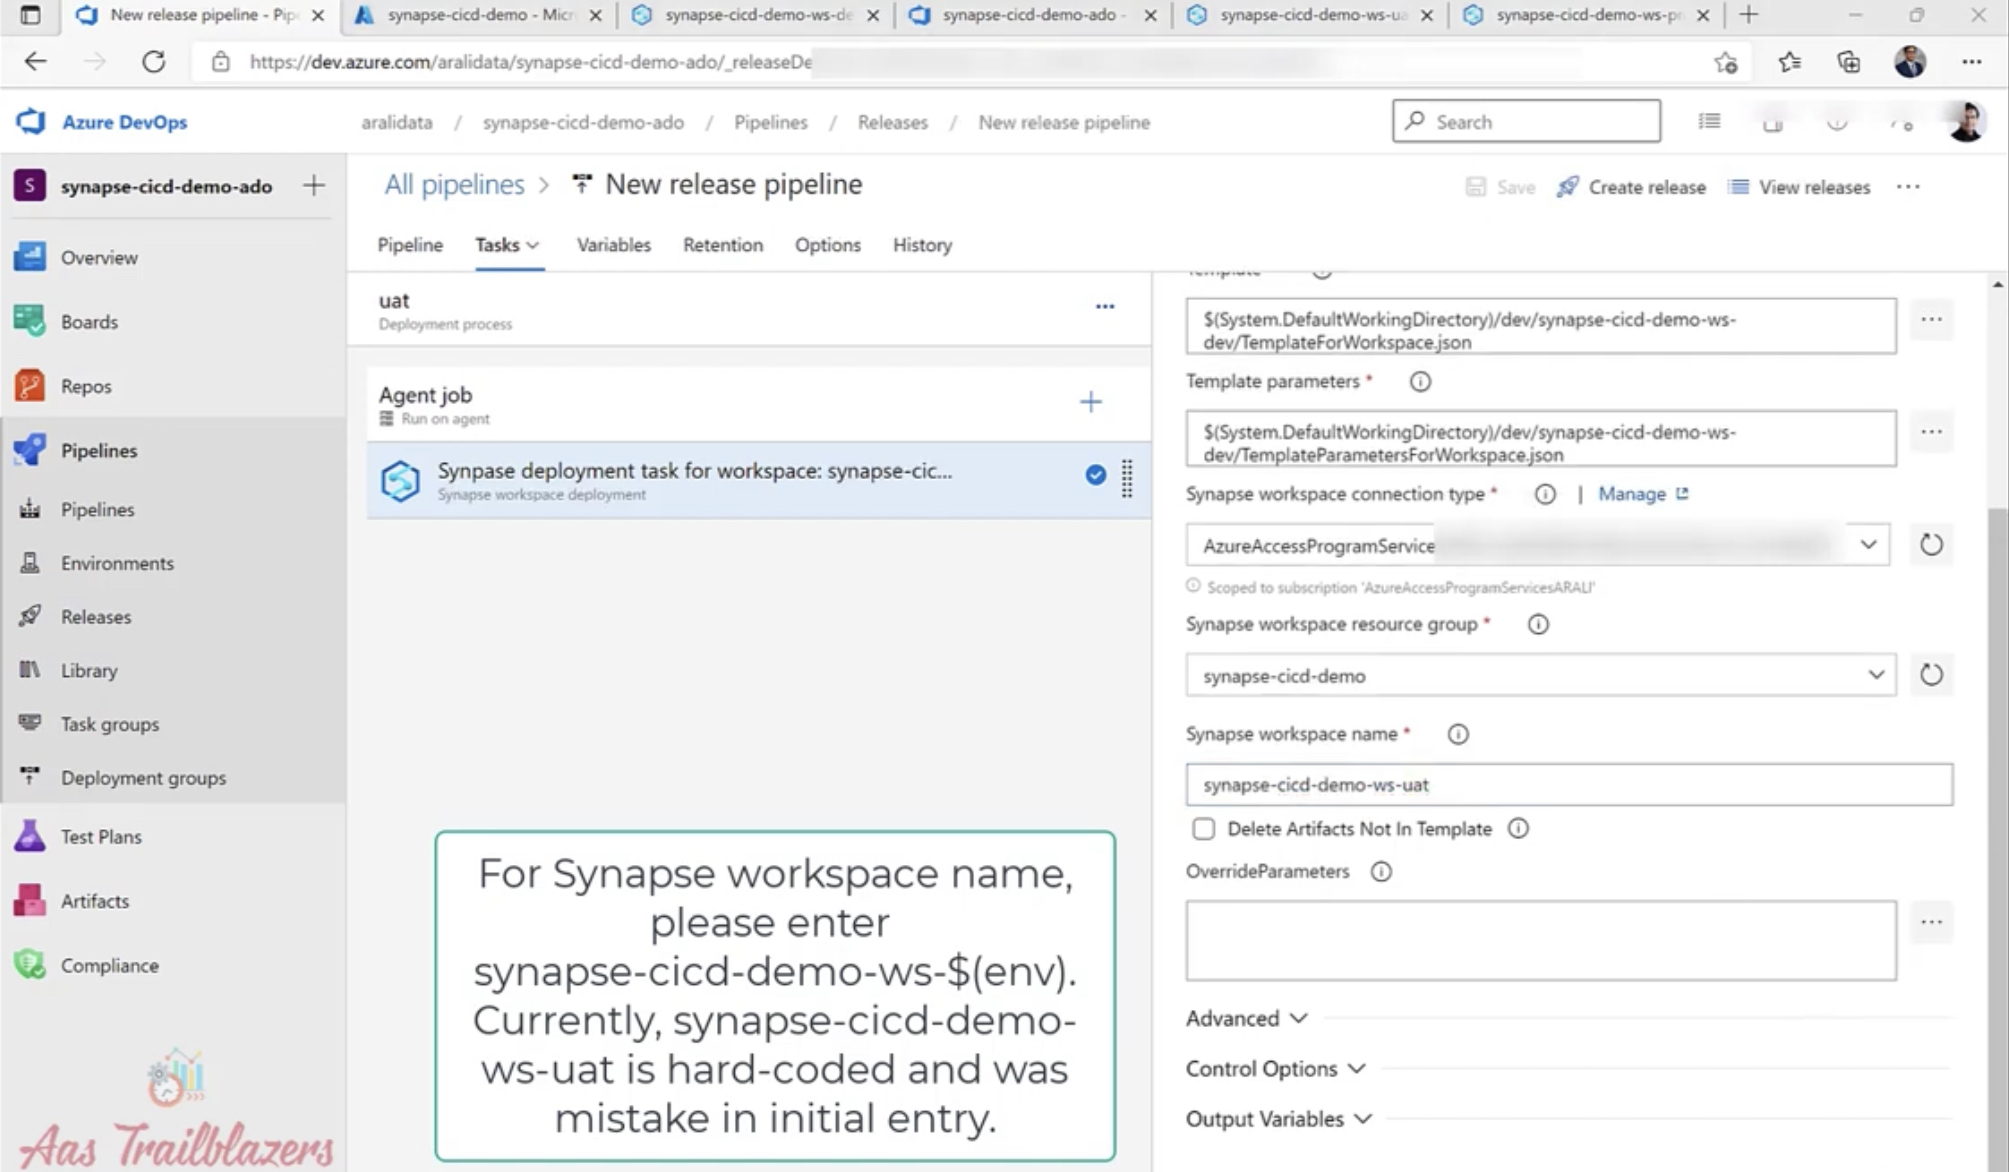
\includegraphics[scale = 0.2]{attachment/chapter_2/Scc161}
	\caption{Setup Stage 1}
\end{figure}
In der Stage 1 zusätzlich zum Artifact genaue Bestandteile des Artifacts hinterlegt. Dazu kommen noch weiter Konfiguration (z.B.: Ressource Gruppe, Subscription).

The name for the workspace, can also be drawn from the pipeline variable
\begin{lstlisting}[style=CMD]
	synapse_cid_demo-ws-${env}	
\end{lstlisting}
In the picture it is hard coded.

In the section \textbf{Overwrite Parameters} we can set different values for the parameters in the parameter artifact file.


\subsection{Besonderheiten}
\begin{itemize}
	\item Ressourcen in allen Bereichen müssen gleich sein: Zum Beispiel muss ein Spark Pool in der Test sowie Produktionsumgebung vorhanden sein, sonst wird ein Fehler ausgewiesen.
	\item Für die Pipeline müssen die Berechtigungen im Test sowie Produktionsbereich gesetzt werden, dass dort eine Artifakt hin einpubiziert wird. Die Roll des Artifakt Publisher wird für den Service Prinzipal benötigt, welcher Zugriff auf den Workspace benötigt
	\begin{figure}[H]
	\centering
	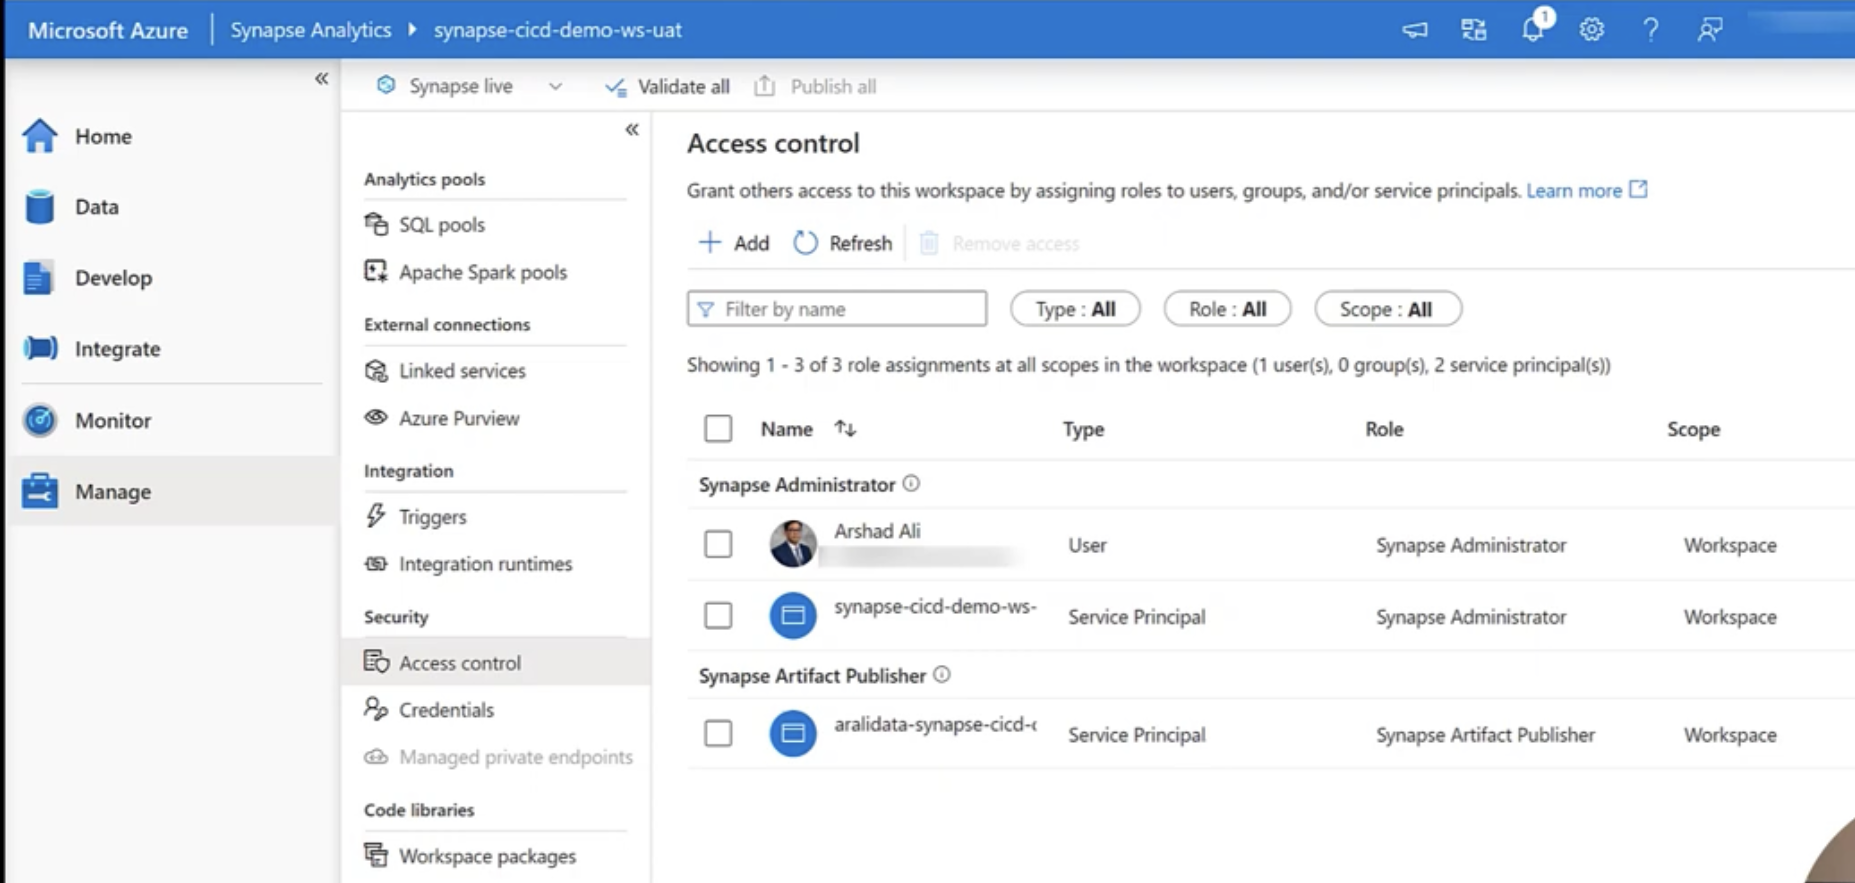
\includegraphics[scale = 0.2]{attachment/chapter_2/Scc162}
	\caption{Roll Asignment}
\end{figure}
\end{itemize}
